\documentclass[a4paper,oneside,BCOR12.5mm,DIV12]{scrartcl} %scrartcl

% Klemmmappen-Korrektur: BCOR8.25mm

% Schnellhefter-Korrektur: BCOR12.5mm

\usepackage{scrpage2}



%\usepackage[polutonikogreek,ngerman]{babel}

\usepackage{ngerman}

\usepackage[latin1]{inputenc}

\usepackage{icomma}

\usepackage{rotating}

\usepackage{units}

%\usepackage{psfrag}

%\usepackage{subfigure}



%%%%%%%%%%%%%%%%%%%%%%%%%%%%

% nur sofern ben�tigt:

%\usepackage{float}

%\restylefloat{figure}

%%%%%%%%%%%%%%%%%%%%%%%%%%%%



\usepackage{amsmath,amssymb,amstext}

\usepackage{graphicx}% f�r Graphiken



\newcommand{\grad}{\ensuremath{^\circ}}

\newcommand{\glref}[1]{Gl.\,\eqref{#1}}

\newcommand{\eqtag}{\stepcounter{equation}\tag{\theequation}}

\newcommand{\abs}[1]{\left|#1\right|}

\newcommand{\bra}[1]{\left(#1\right)}

\newcommand{\NOT}[1]{\overline{#1}}
\newcommand{\OR}{\vee}
\newcommand{\AND}{\wedge}
\newcommand{\EXOR}{~\underline{\OR}~}

\newcommand{\eps}{\ensuremath{\varepsilon}}

%\renewcommand{\phi}{\varphi}

\renewcommand{\epsilon}{\varepsilon}



\title{P1-63,64,65: Schaltlogik\\Vorbereitungshilfe}

\author{Christian Barth (1196701)\\ Christian Benz (1204880)}

\date{09.12.2007}

\pagestyle{scrheadings}

\ihead{P1-63,64,65: Schaltlogik}

\setheadsepline{0.5pt}

\setfootsepline{0.5pt}

\ifoot{}

\ofoot{\pagemark}

\cfoot{}

\begin{document}

\section*{Schaltpl�ne zum Ausschneiden}
\subsection*{1.1 AND-Gatter}
\begin{center}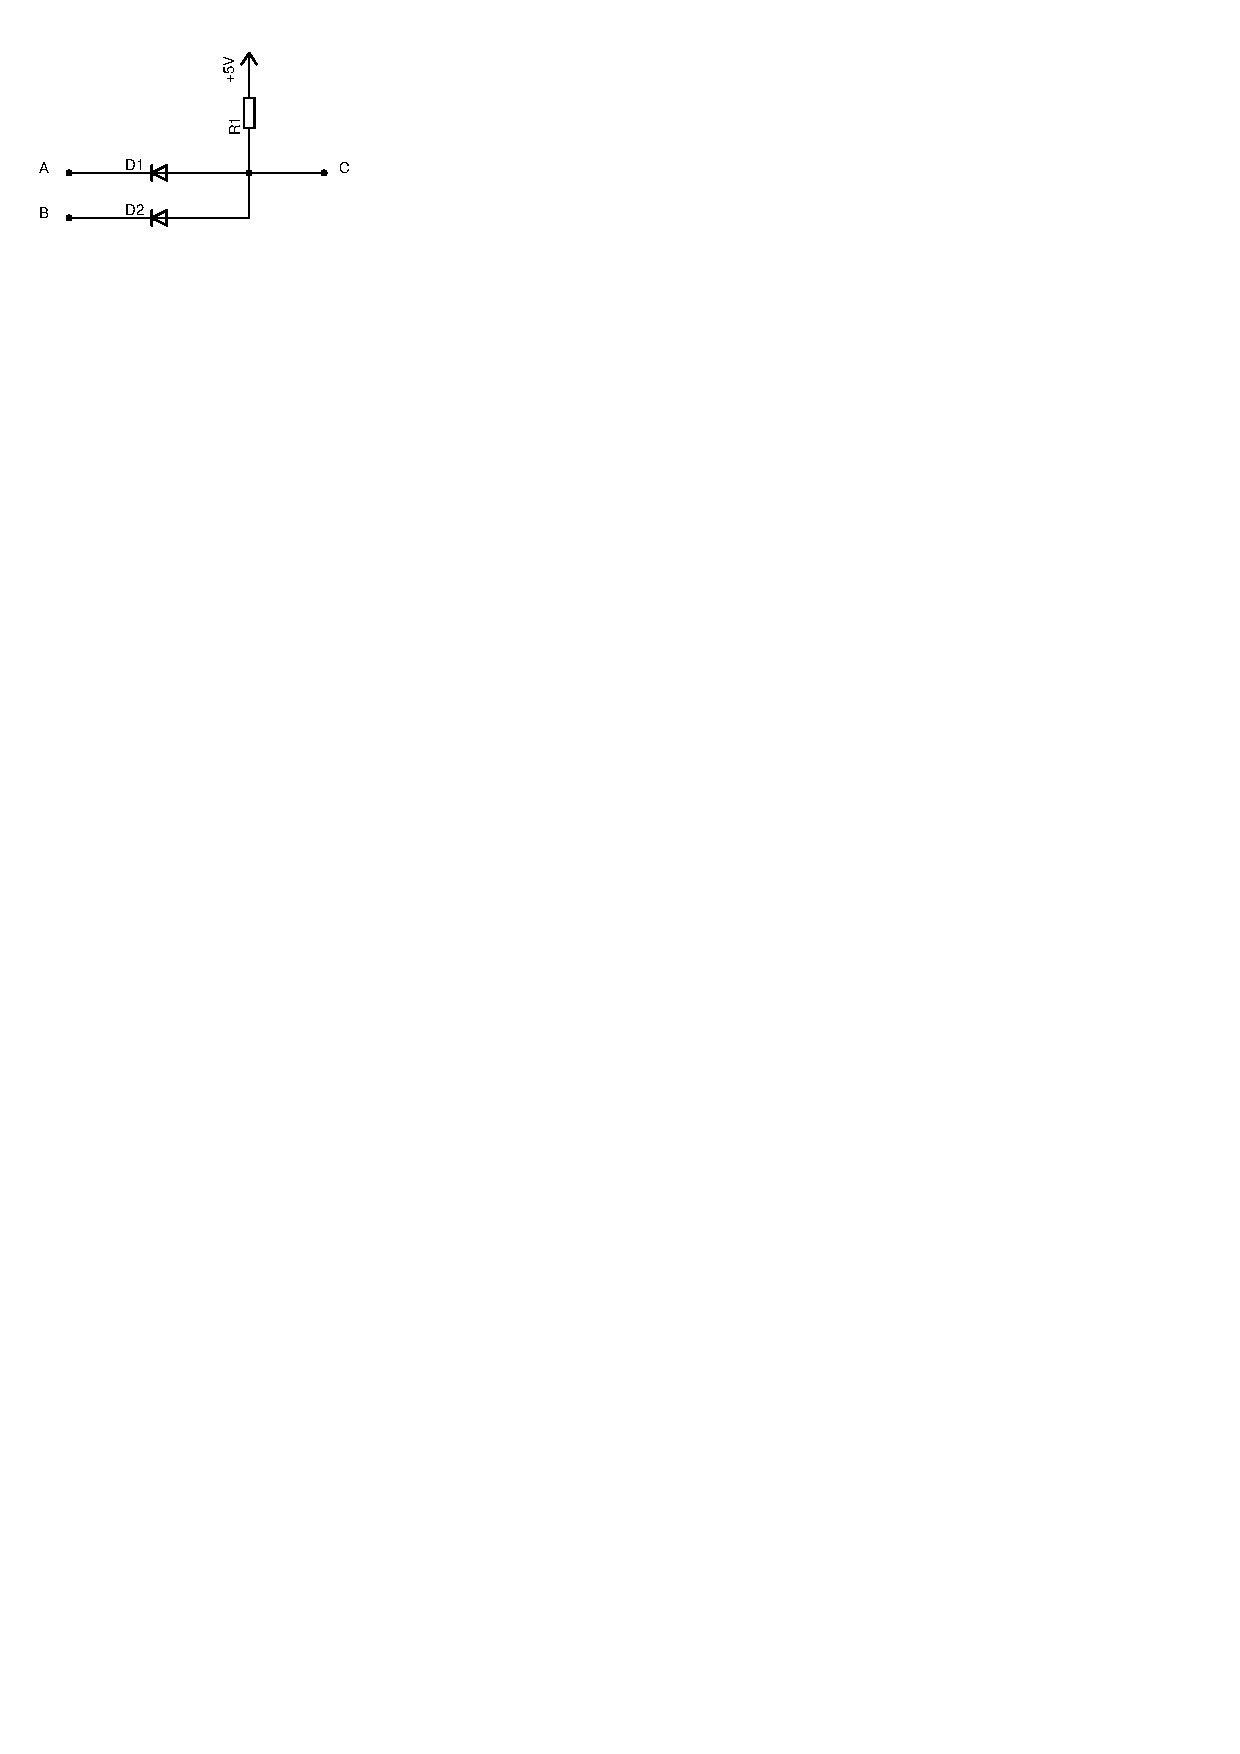
\includegraphics[height=5cm]{Schaltplaene/11_Dioden-AND-Gatter.pdf}\end{center}
\subsection*{1.2 NOT-Gatter}
\begin{center}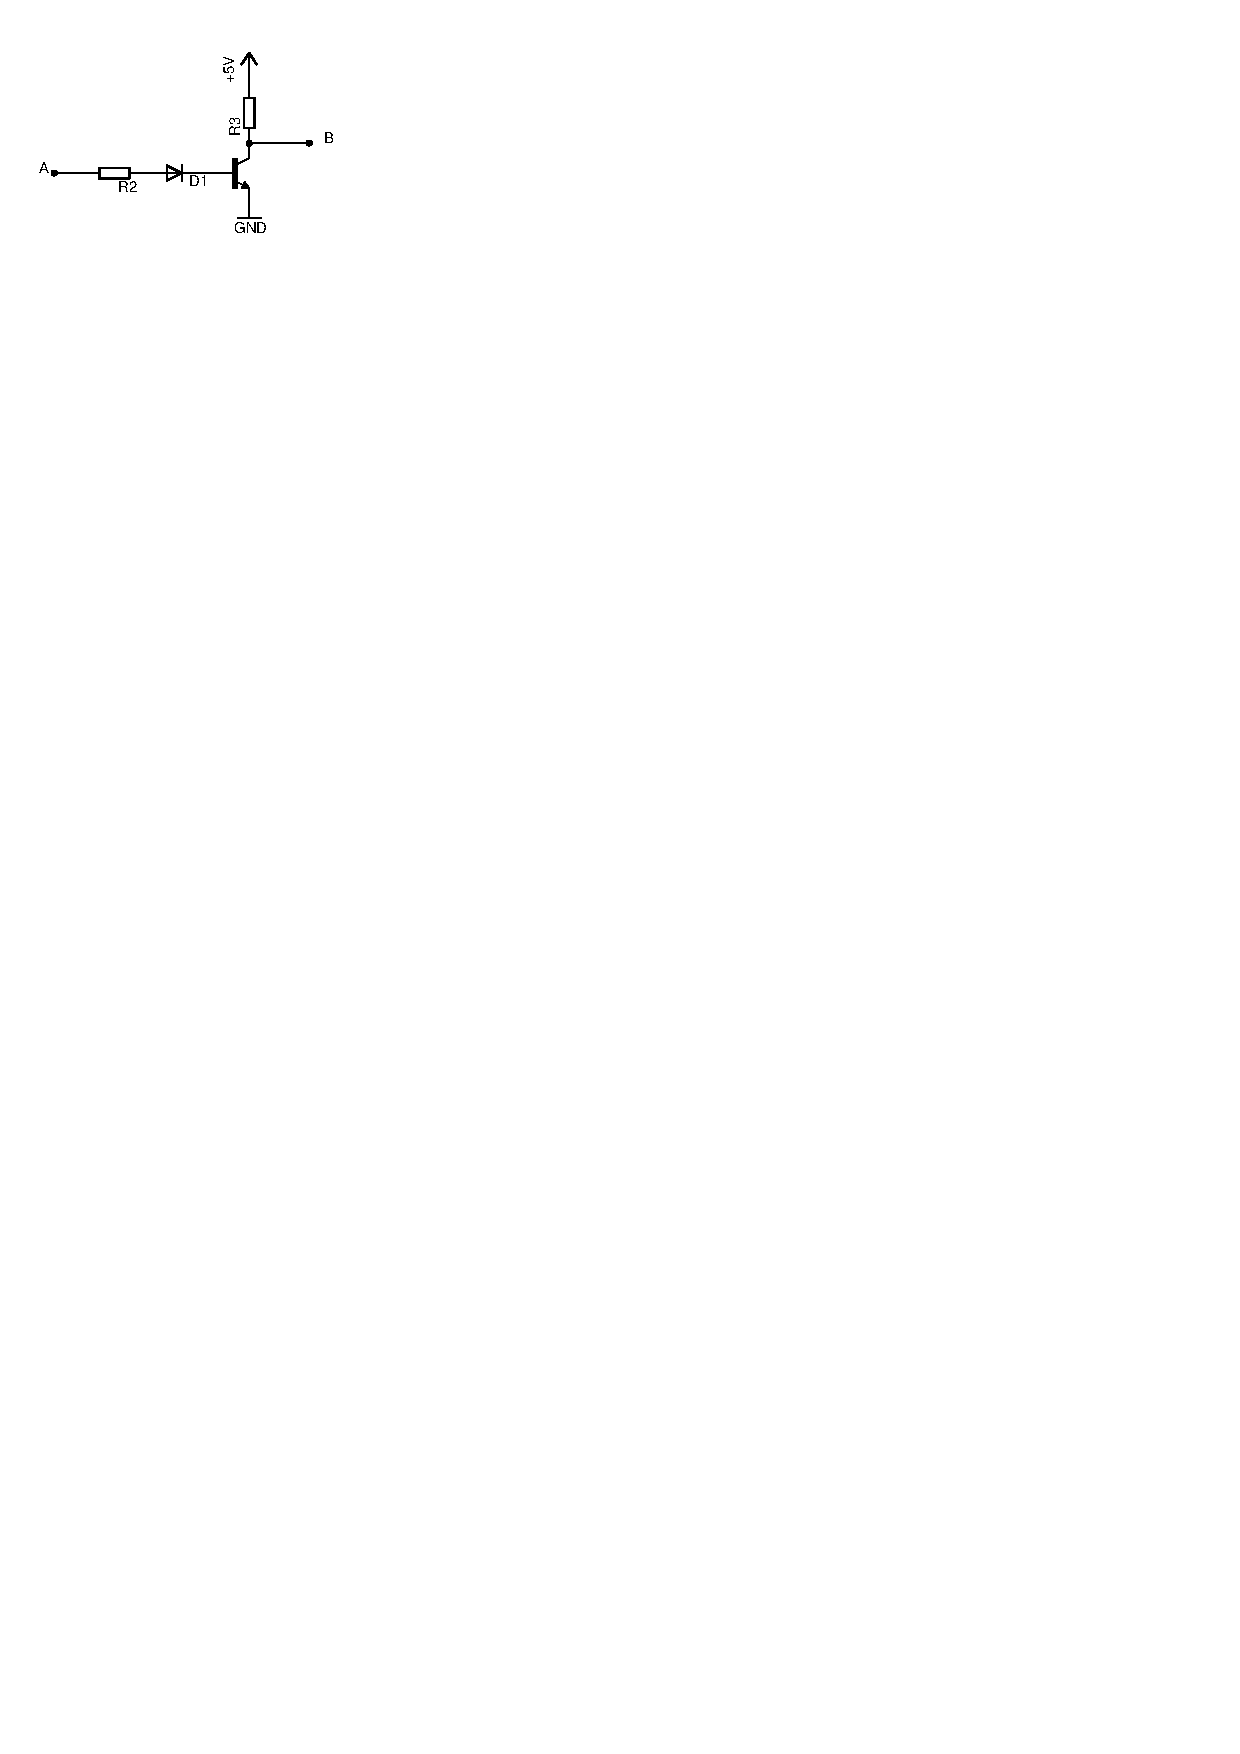
\includegraphics[height=5cm]{Schaltplaene/12a_NOT-Gatter.pdf}\end{center}
\subsection*{1.2 NAND-Gatter}
\begin{center}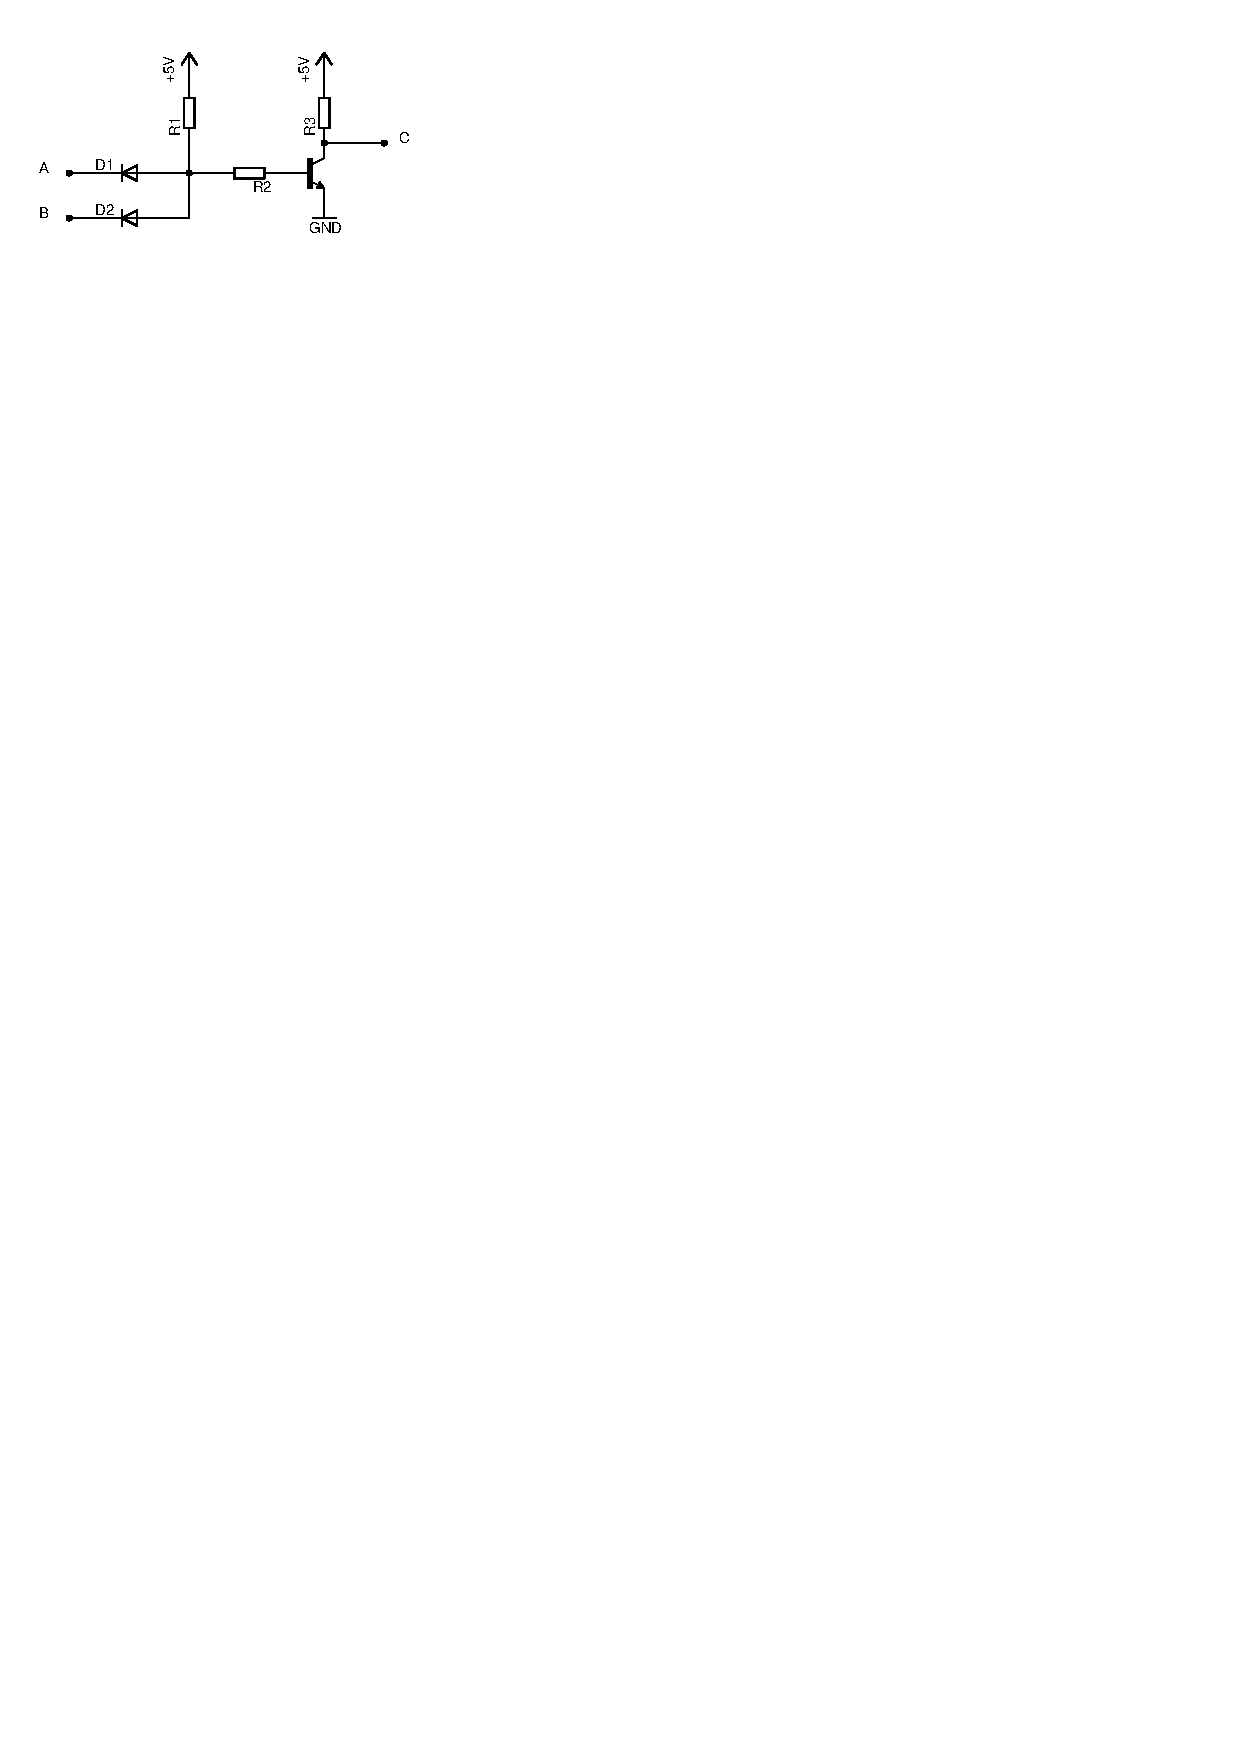
\includegraphics[height=5cm]{Schaltplaene/12b_NAND-Gatter.pdf}\end{center}
\subsection*{1.3 OR-Gatter}
\begin{center}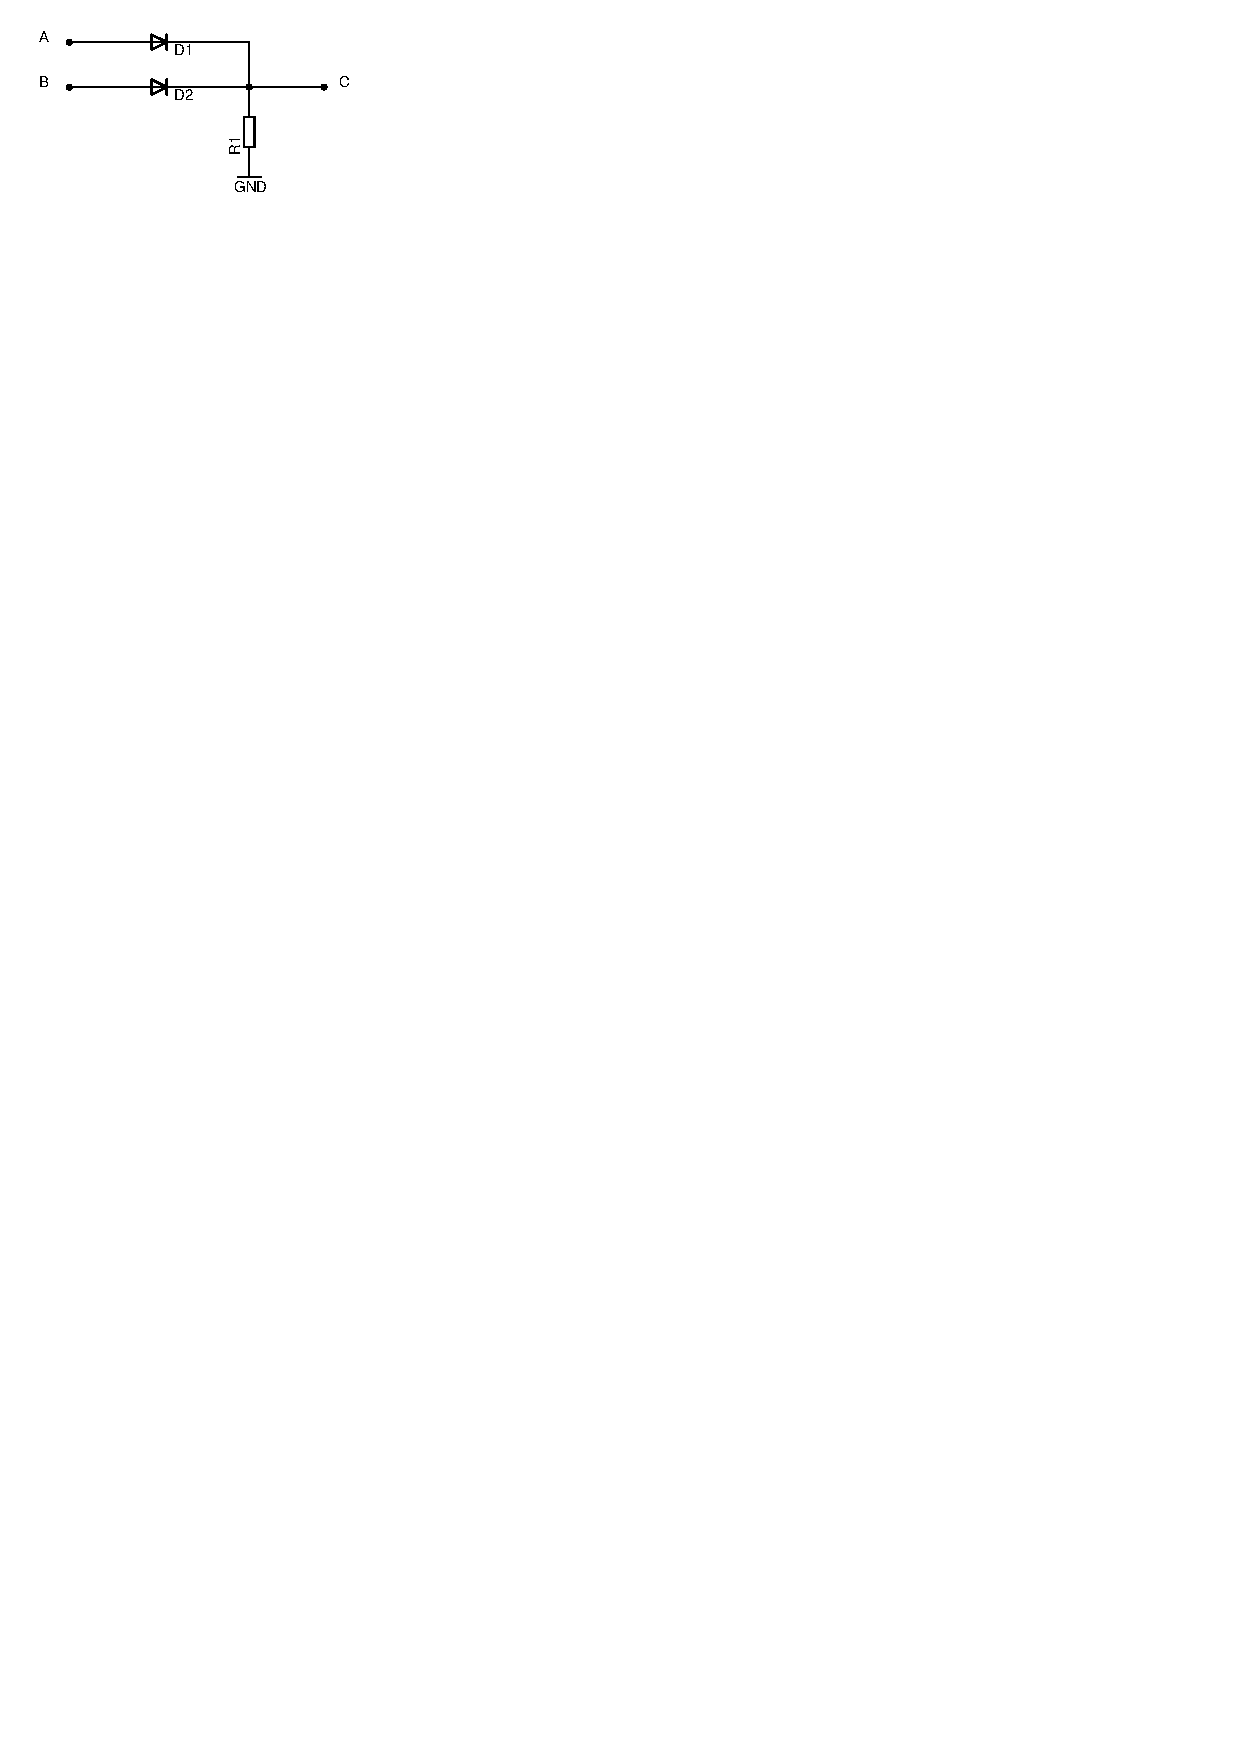
\includegraphics[height=5cm]{Schaltplaene/13_Dioden-OR-Gatter.pdf}\end{center}
\subsection*{2 Weitere einfache logische Funktionen (Gatter), realisiert mit ICs}
\begin{center}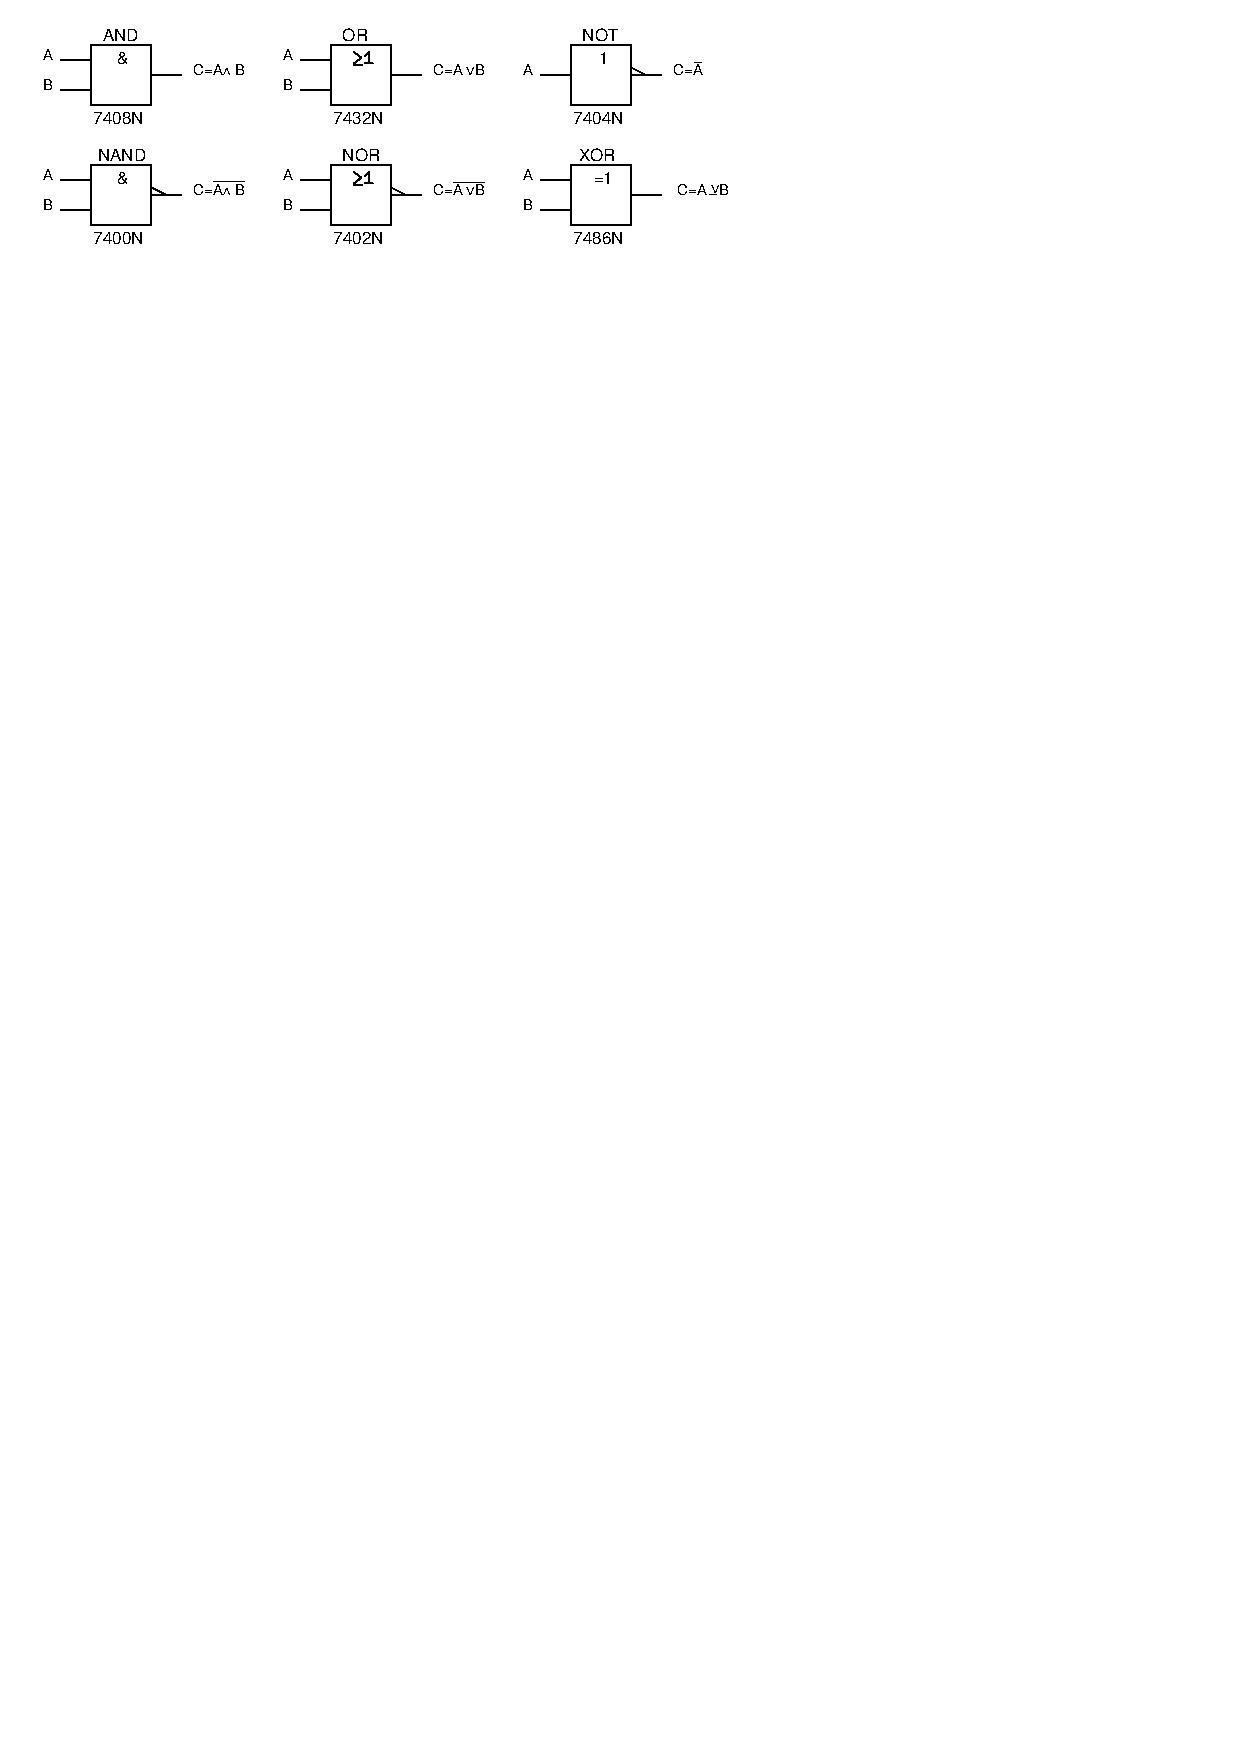
\includegraphics[height=4cm]{Schaltplaene/10_Schaltsymbole.pdf}\end{center}
\subsection*{2.1 Inverter aus NAND- oder NOR-Gatter}
\begin{center}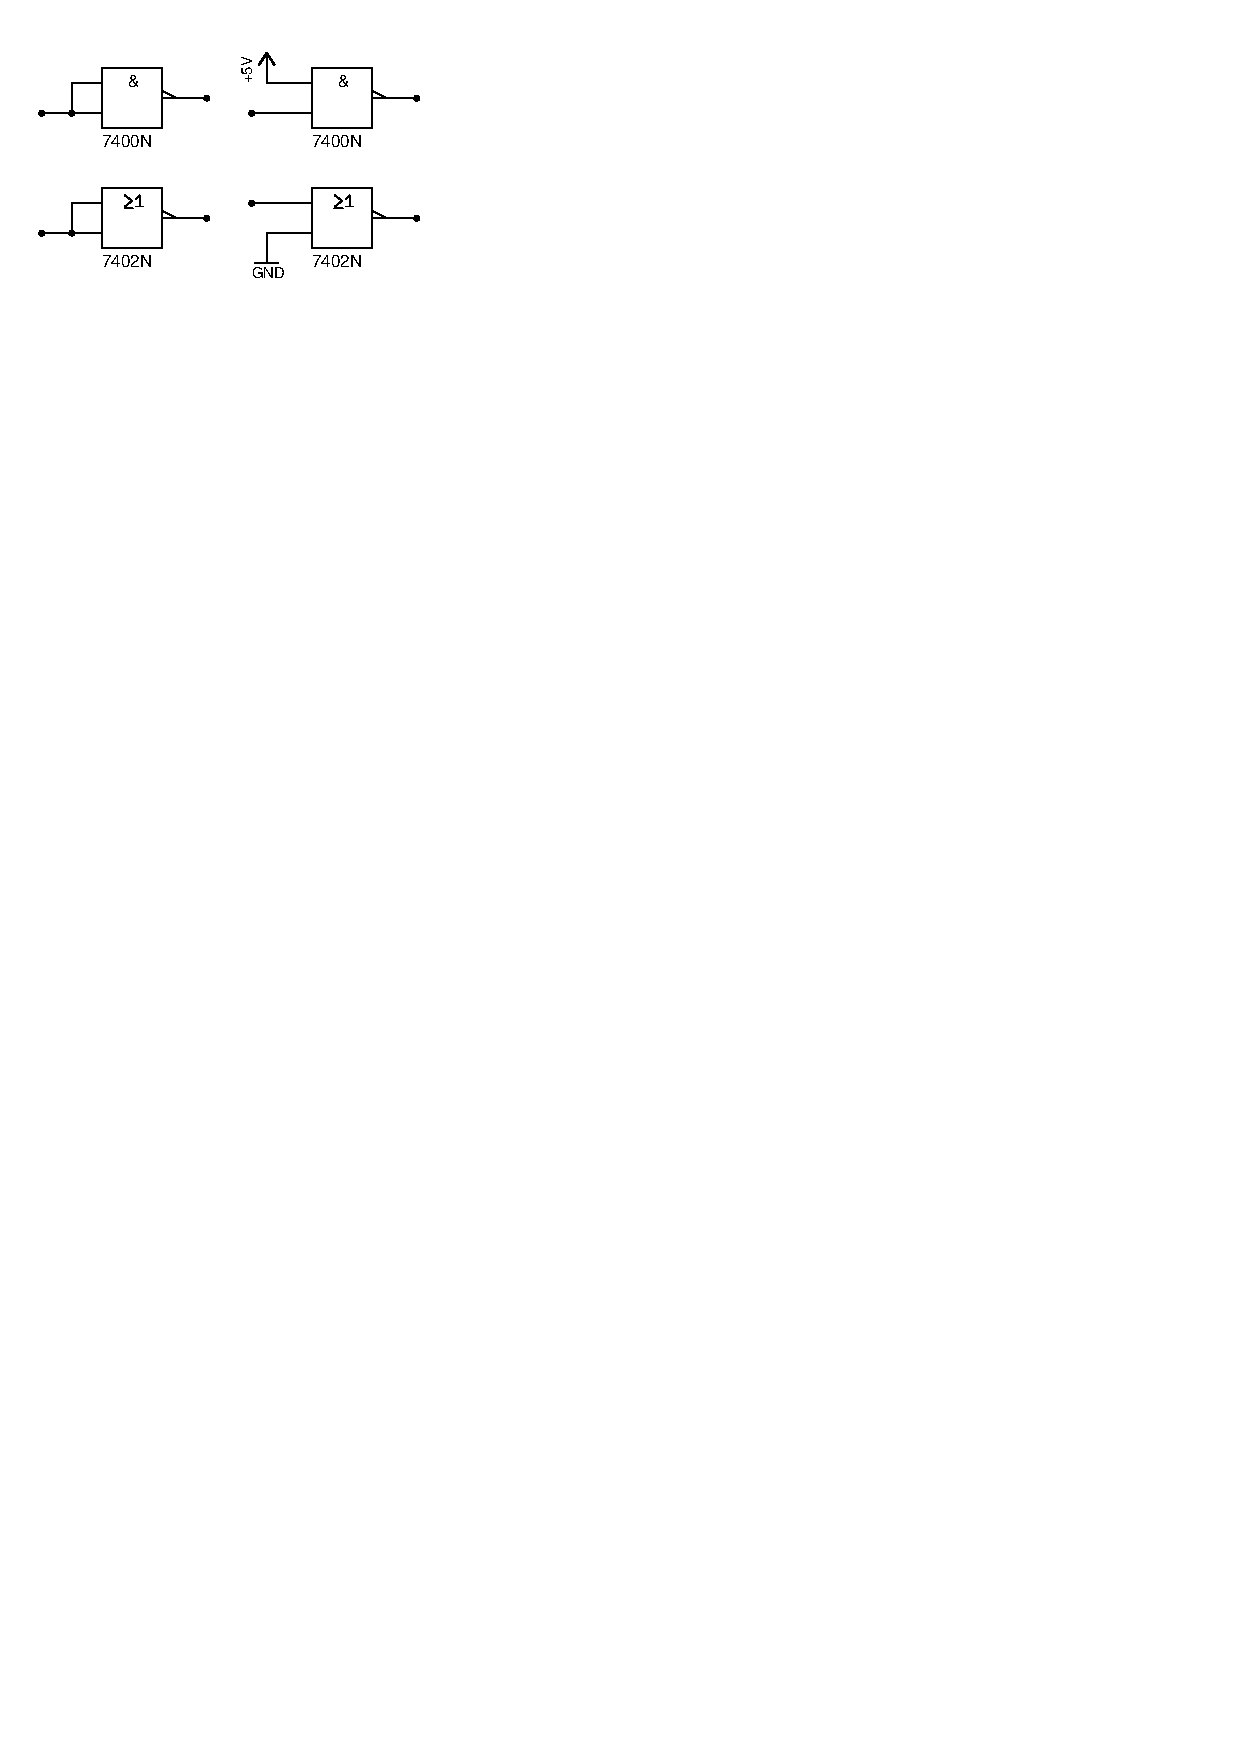
\includegraphics[height=5cm]{Schaltplaene/21_NOT_aus_NAND_oder_NOR.pdf}\end{center}
\subsection*{2.2 EXOR-Gatter}
\begin{center}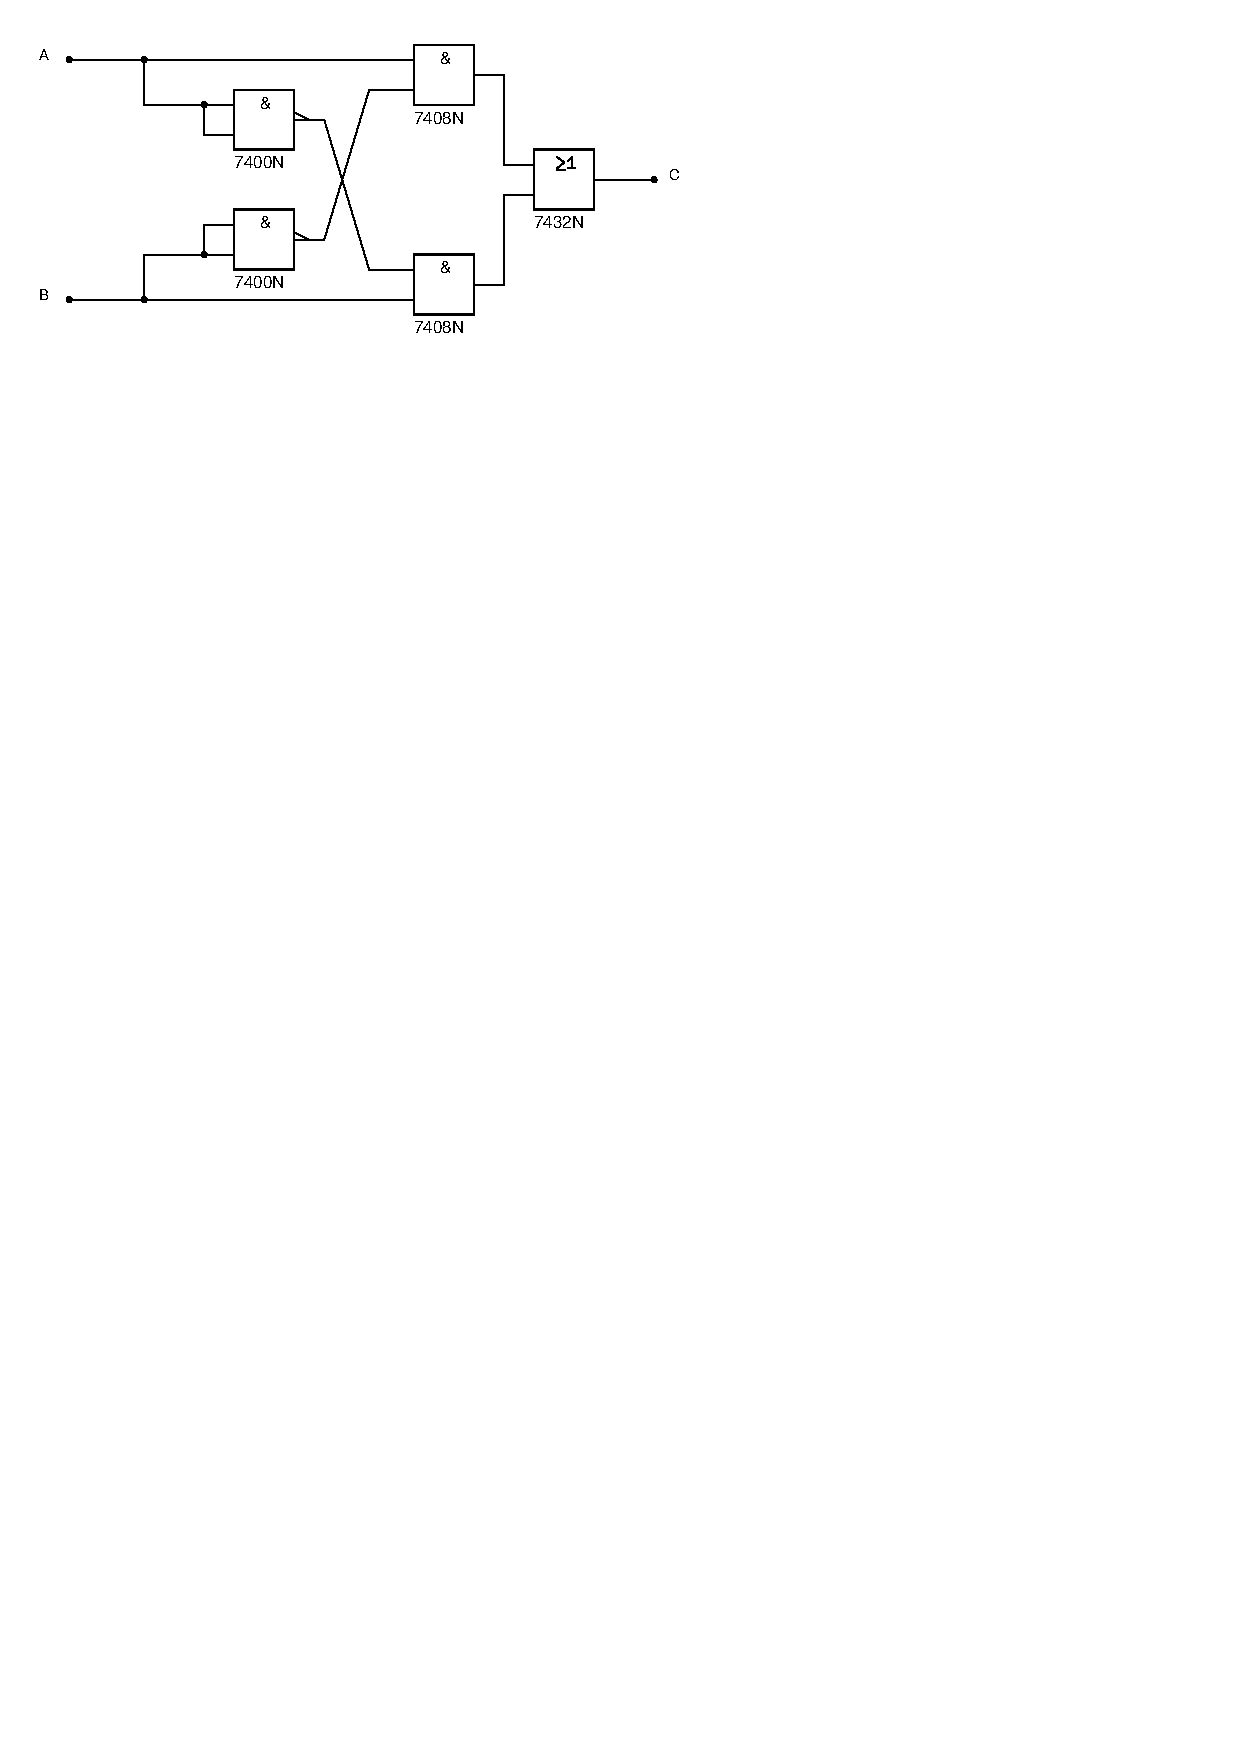
\includegraphics[height=7cm]{Schaltplaene/22_XOR_aus_disjunktiver_Normalform.pdf}\end{center}
\subsection*{2.3 EXOR-Gatter aus NAND-Gatter}
\begin{center}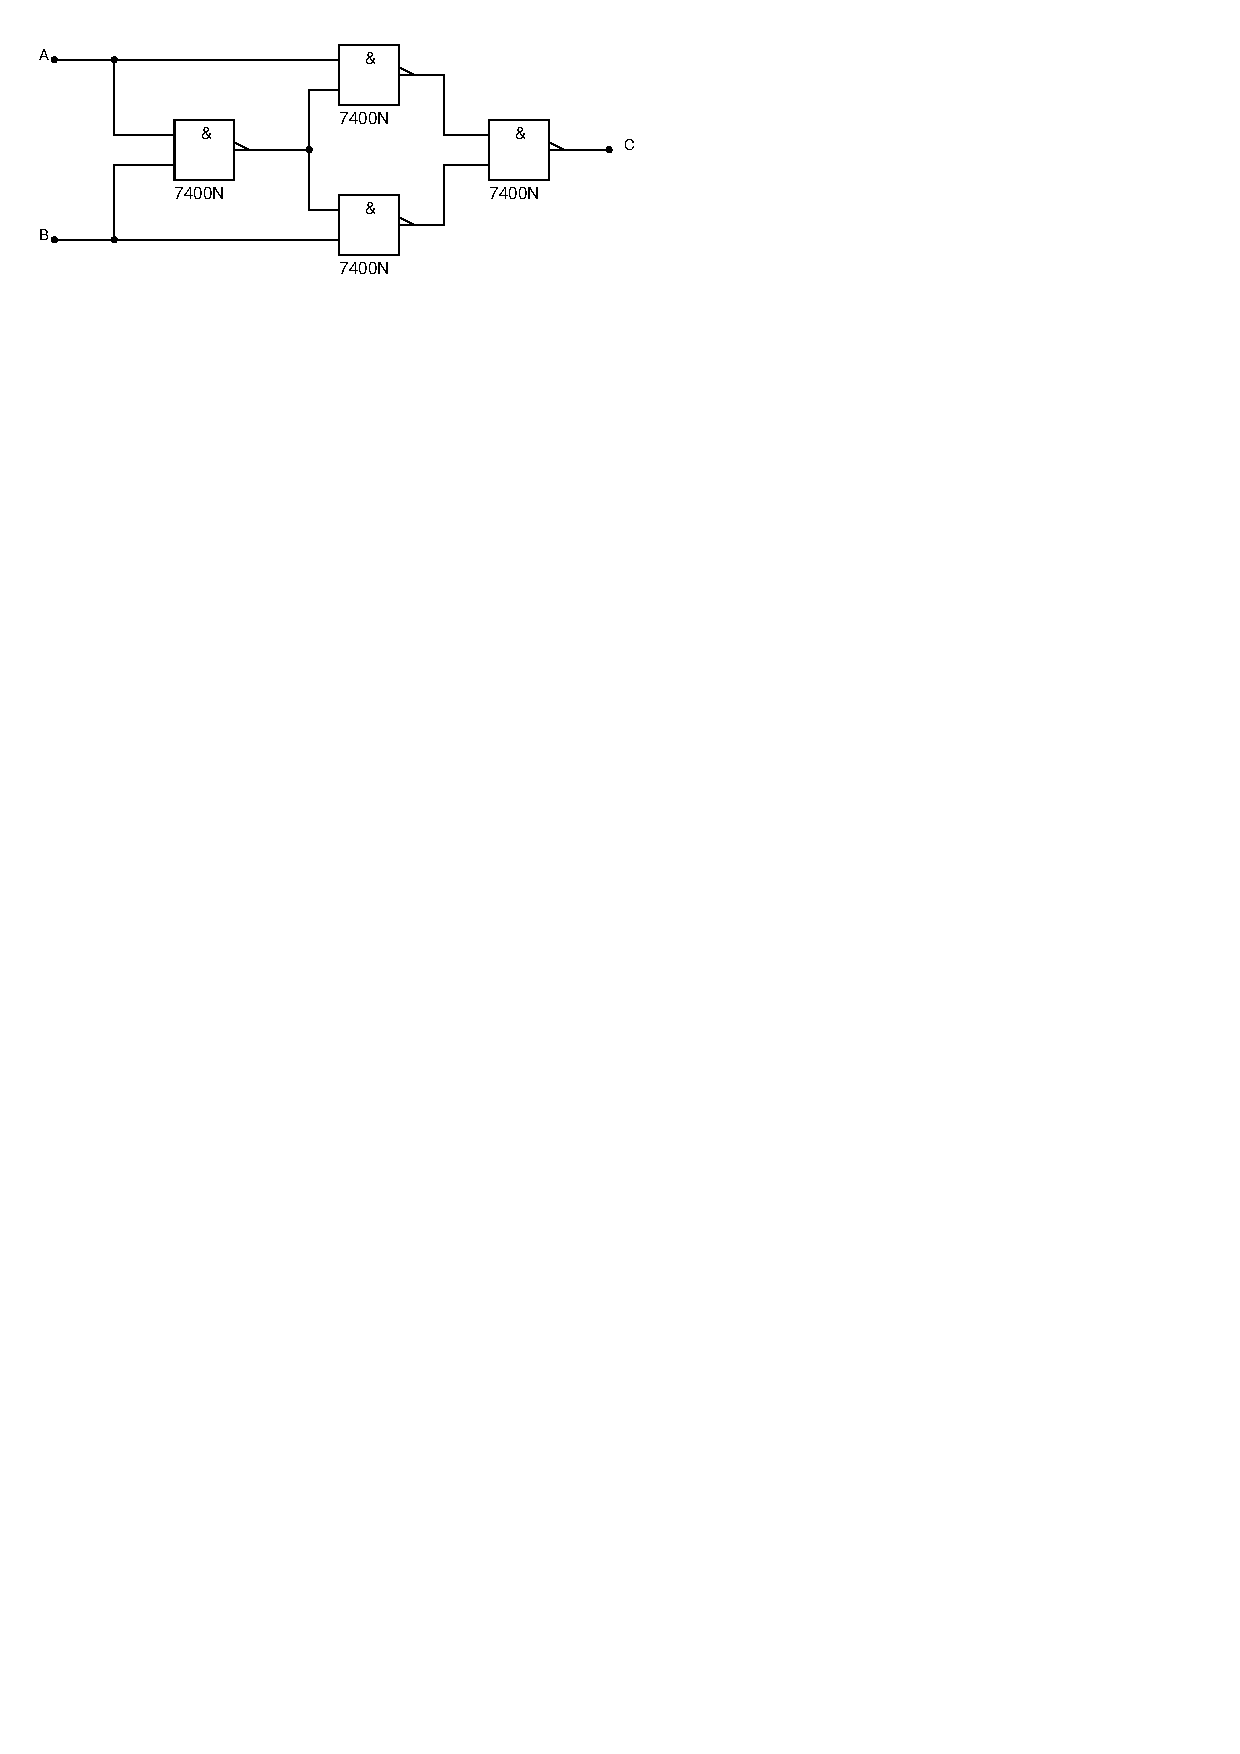
\includegraphics[height=6cm]{Schaltplaene/23_XOR_aus_NAND-Gatter.pdf}\end{center}
\subsection*{3.1 Halbaddierer}
\begin{center}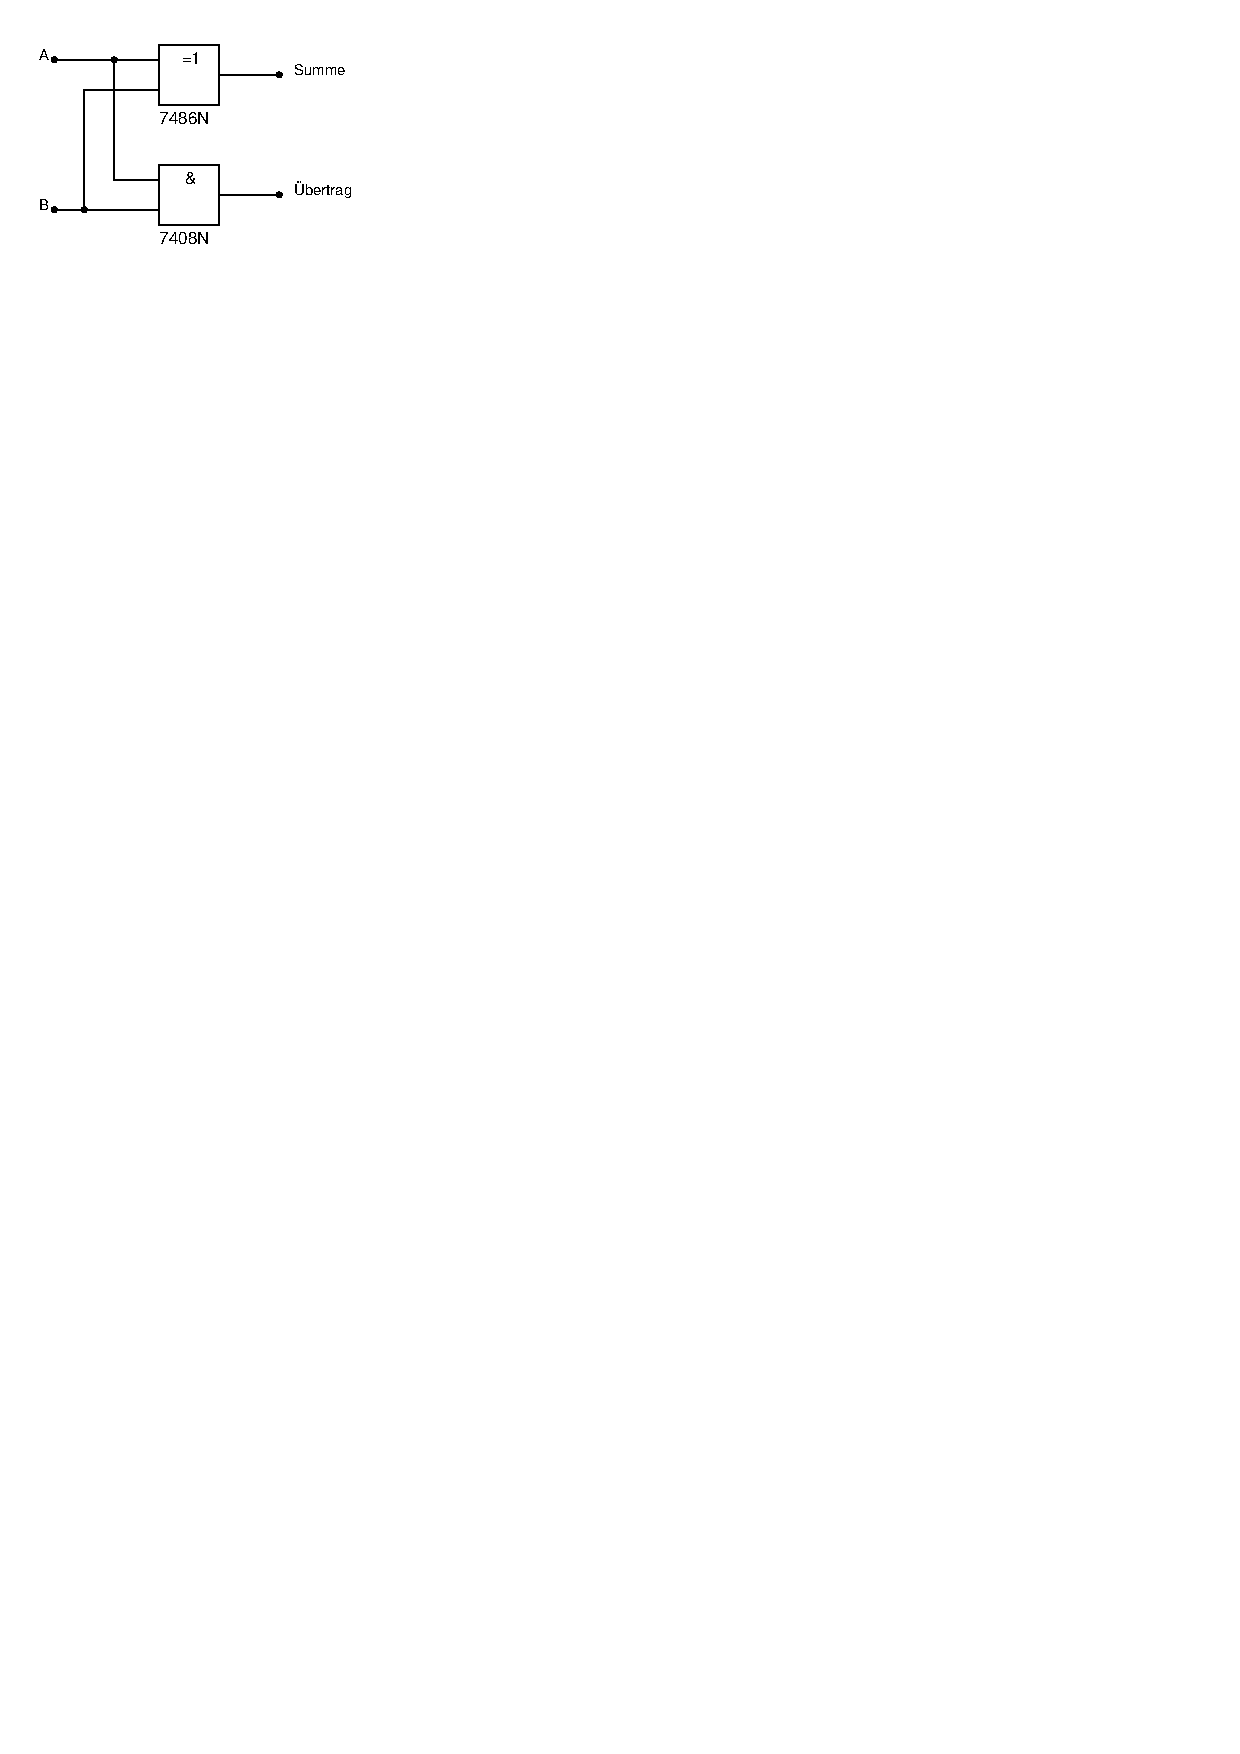
\includegraphics[height=5cm]{Schaltplaene/31_Halbaddierer.pdf}\end{center}
\subsection*{3.2 Volladdierer}
\begin{center}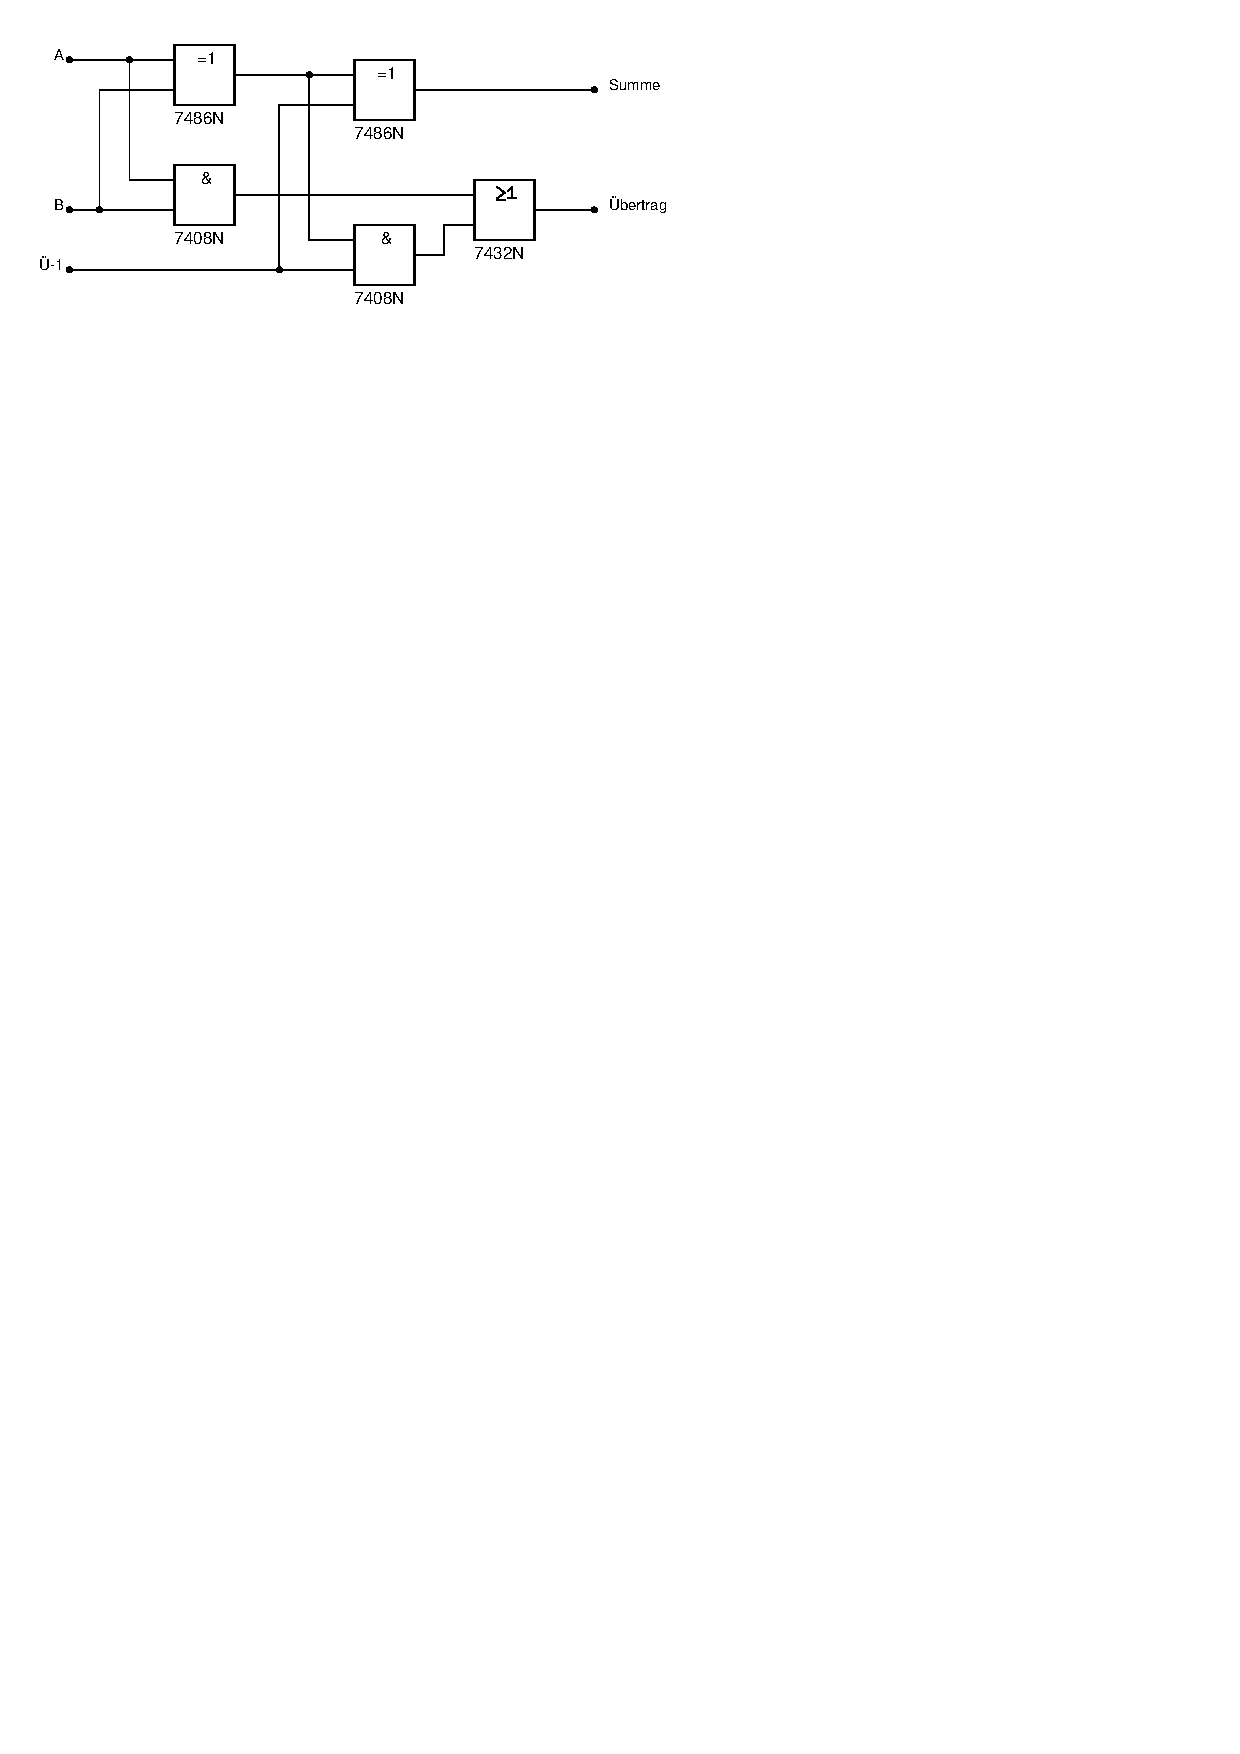
\includegraphics[height=6cm]{Schaltplaene/32_1-Bit-Volladdierer_aus_zwei_Halbaddierern.pdf}\end{center}
\begin{center}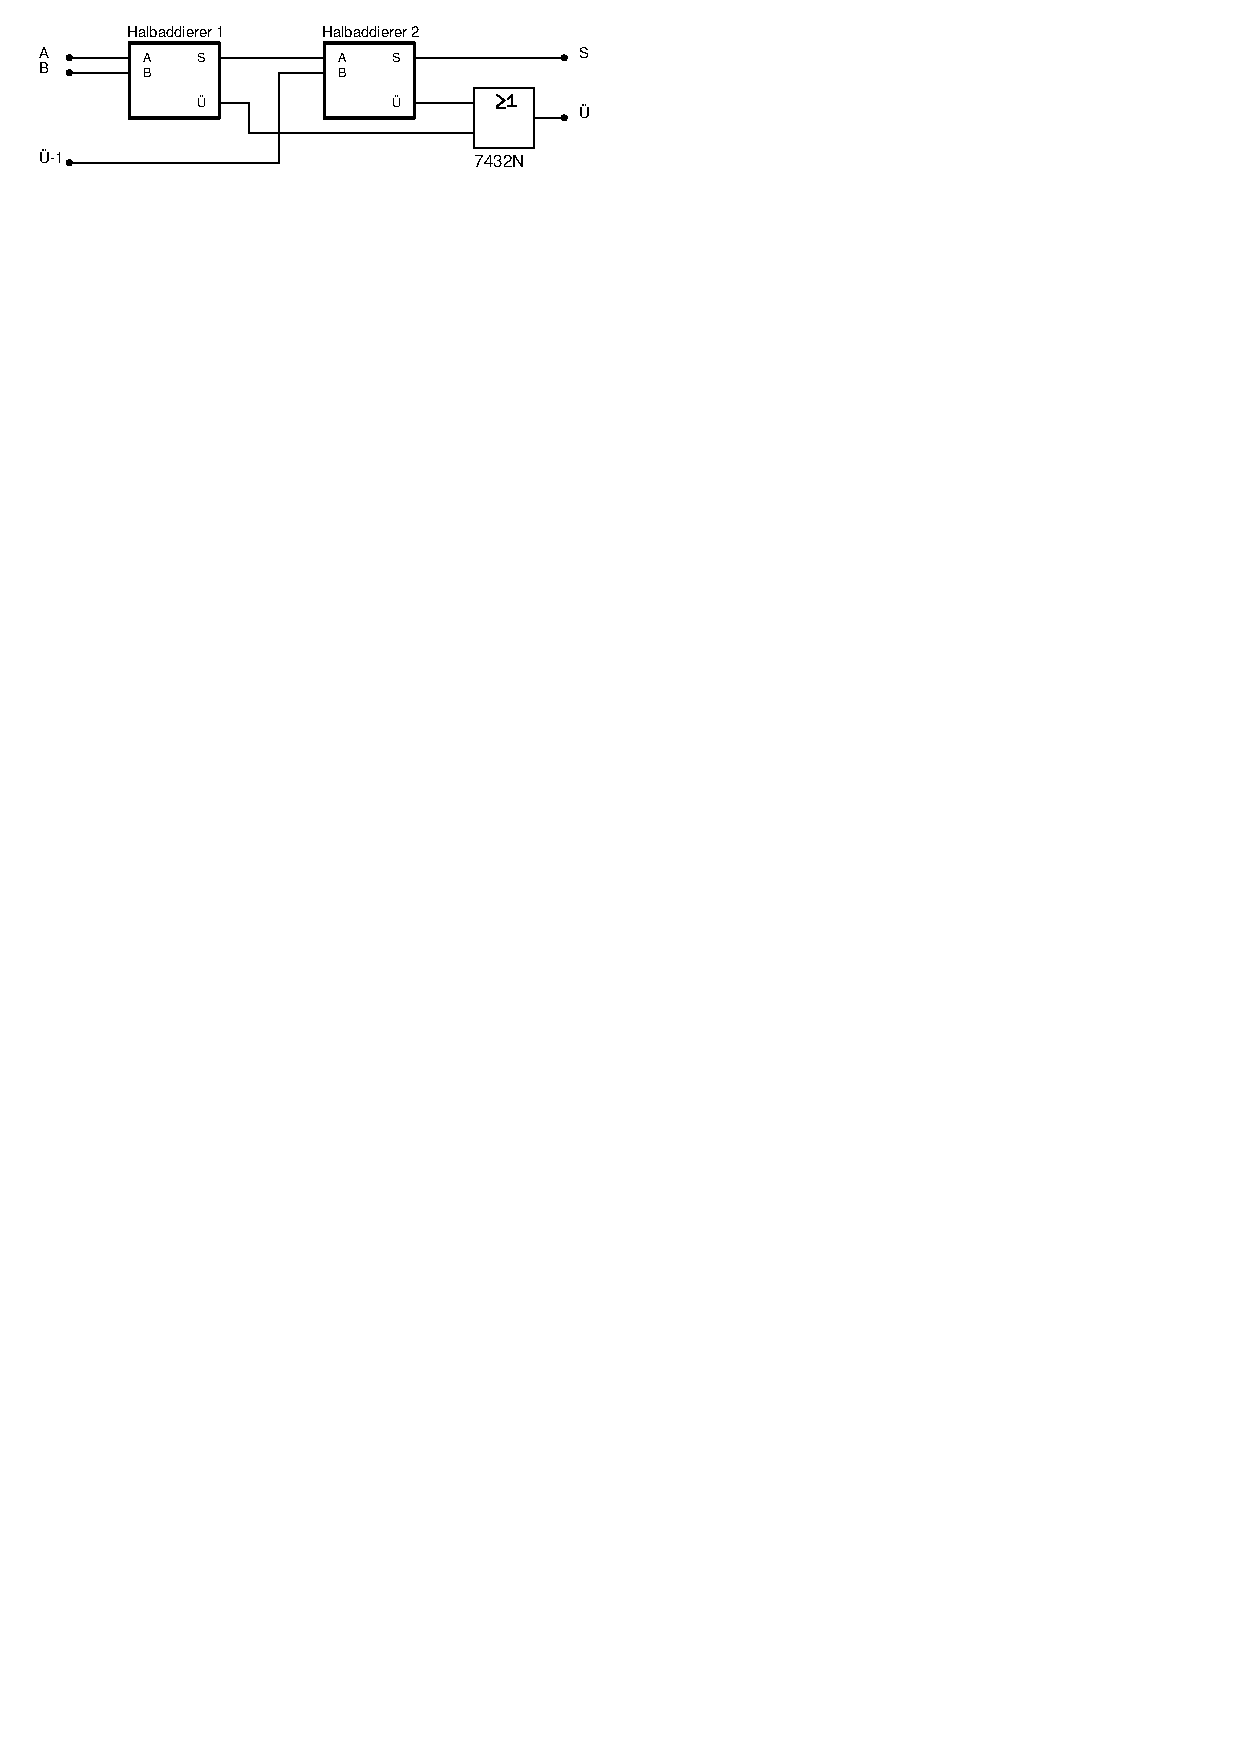
\includegraphics[height=3cm]{Schaltplaene/32b_1-Bit-Volladdierer_aus_zwei_Halbaddierern_einfach.pdf}\end{center}
\begin{center}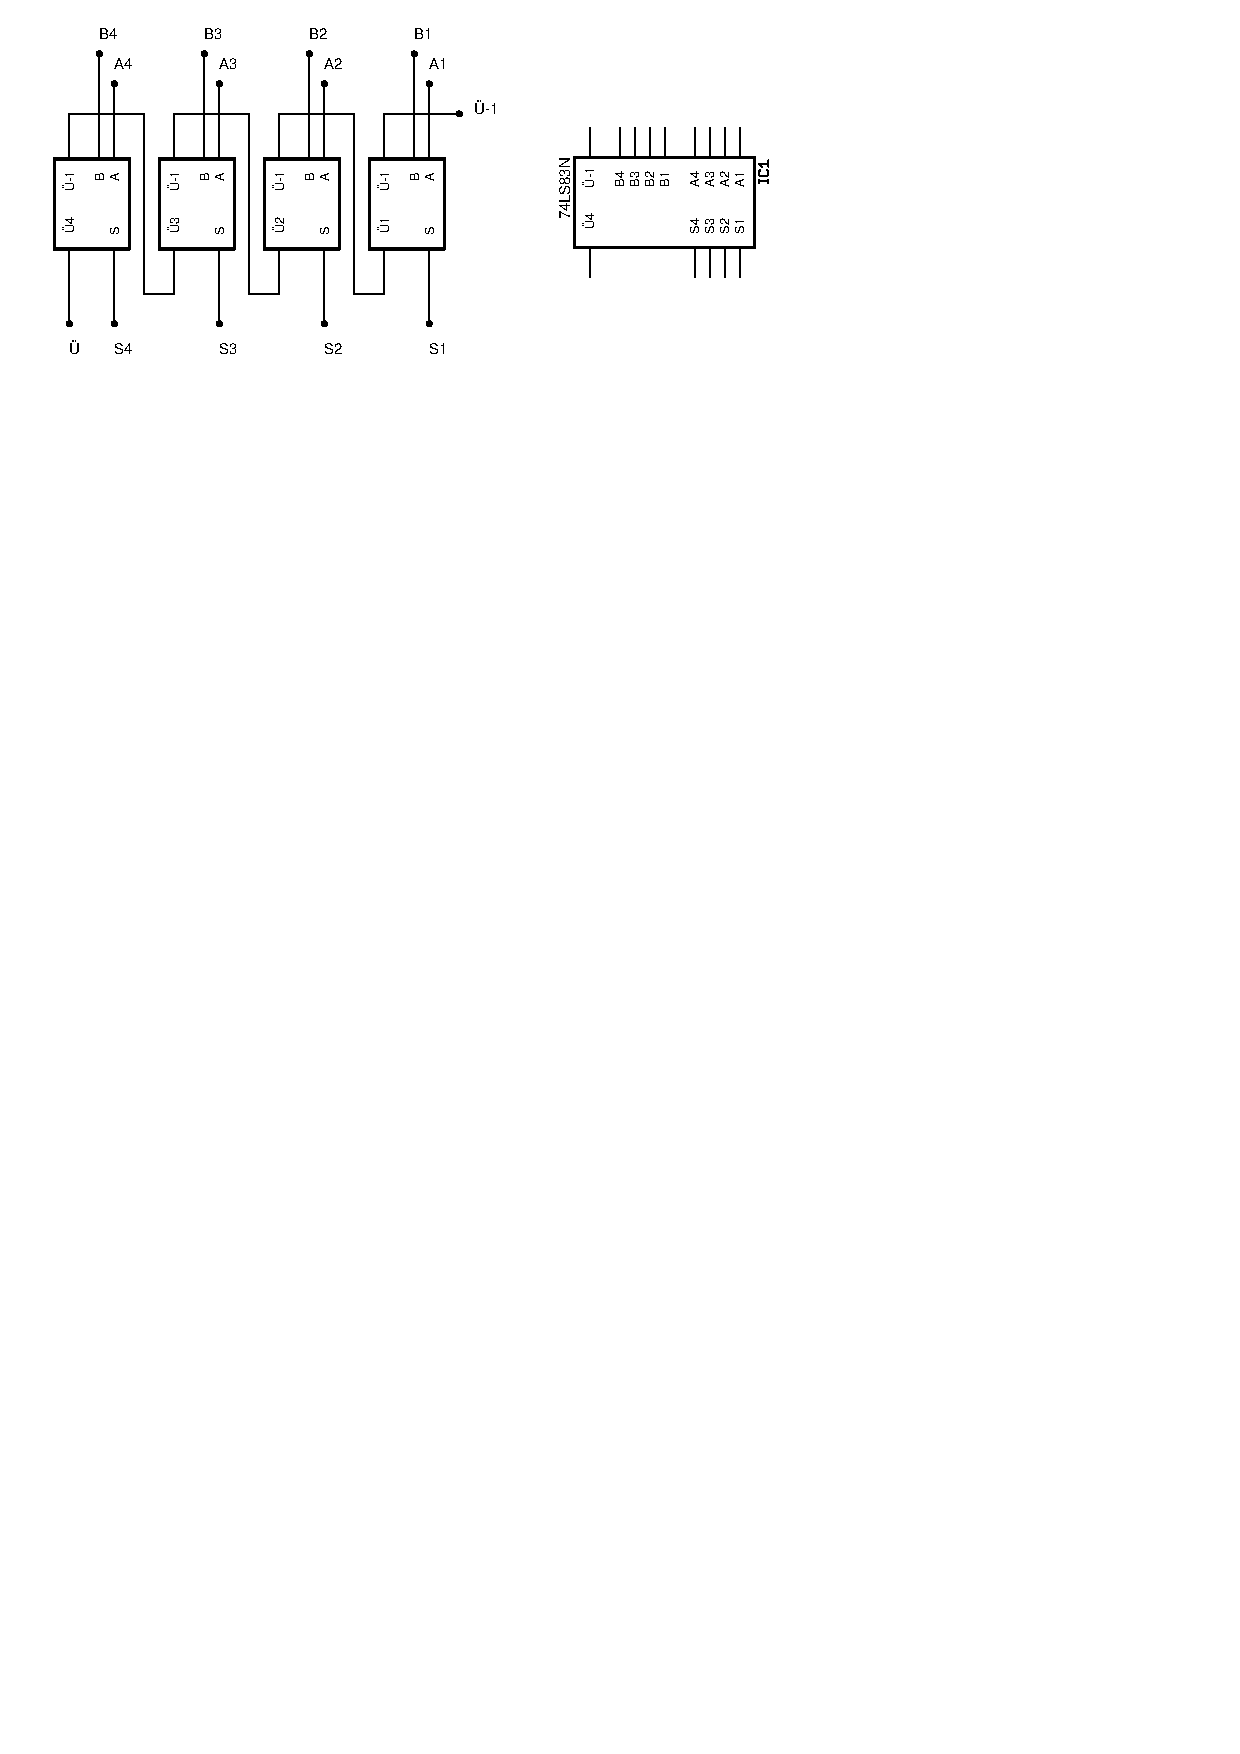
\includegraphics[height=7cm]{Schaltplaene/32c_4-Bit_Volladdierer.pdf}\end{center}
\subsection*{3.3 Subtrahierer}
\begin{center}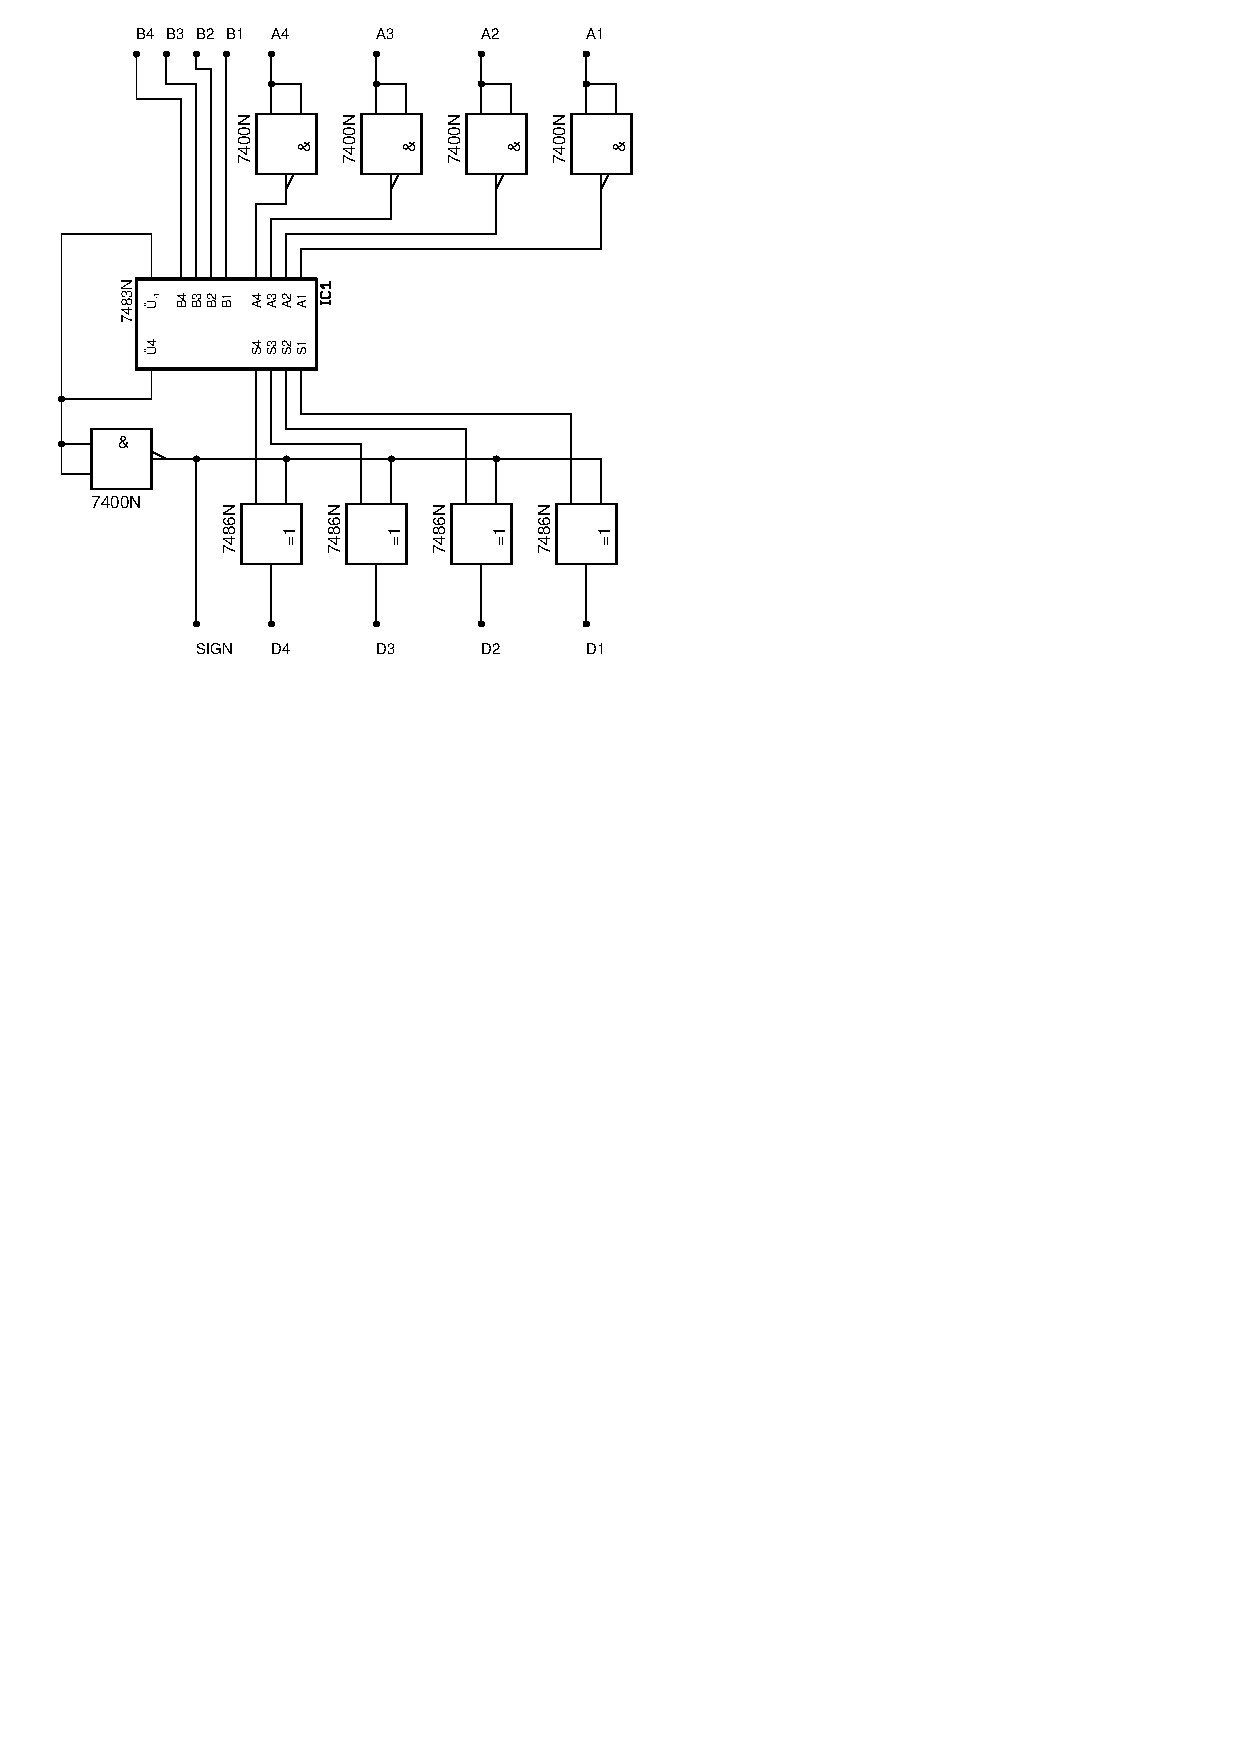
\includegraphics[height=11cm]{Schaltplaene/33_Subtrahierer.pdf}\end{center}
\subsection*{4.1 RS-Flip-Flop}
\begin{center}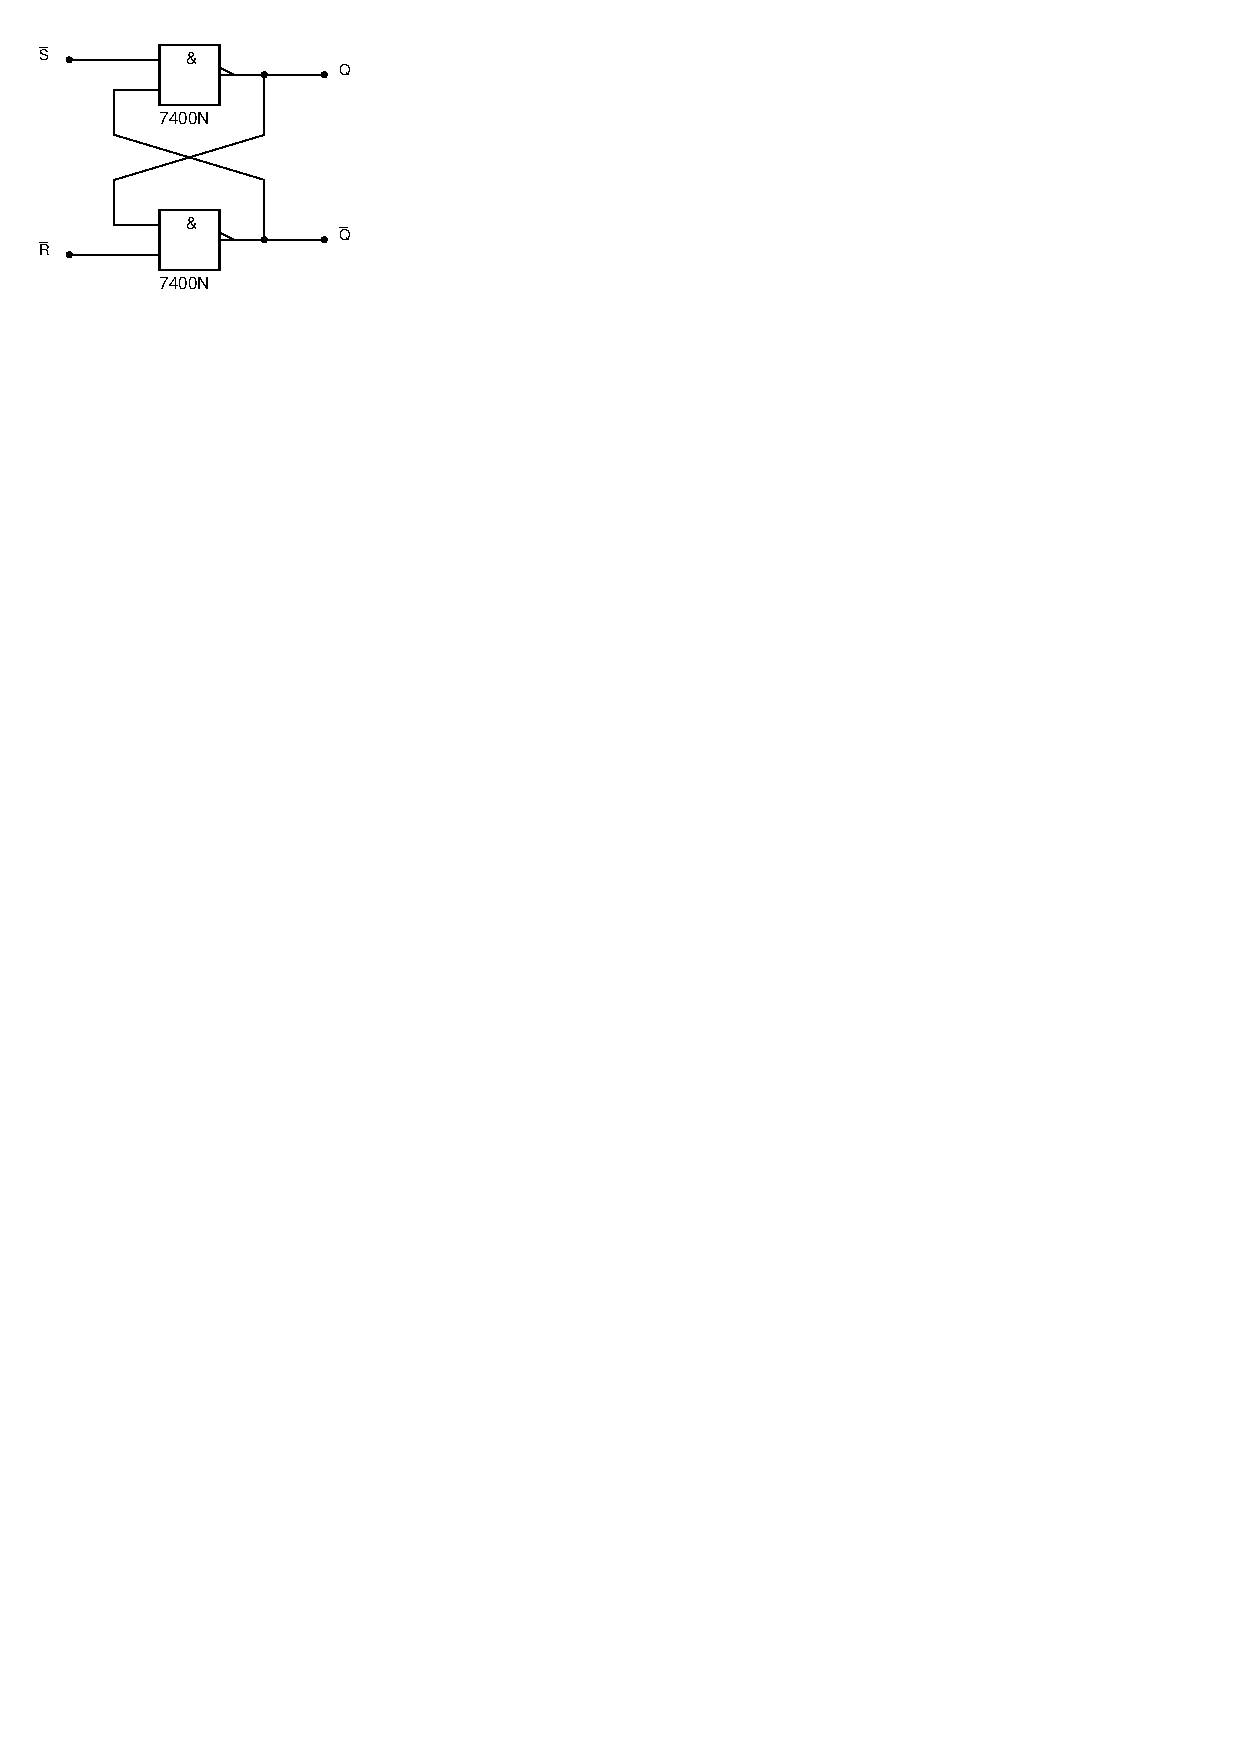
\includegraphics[height=6cm]{Schaltplaene/41_RS-Flip-Flop.pdf}\end{center}
\subsection*{4.2 Getaktetes RS-Flip-Flop}
\begin{center}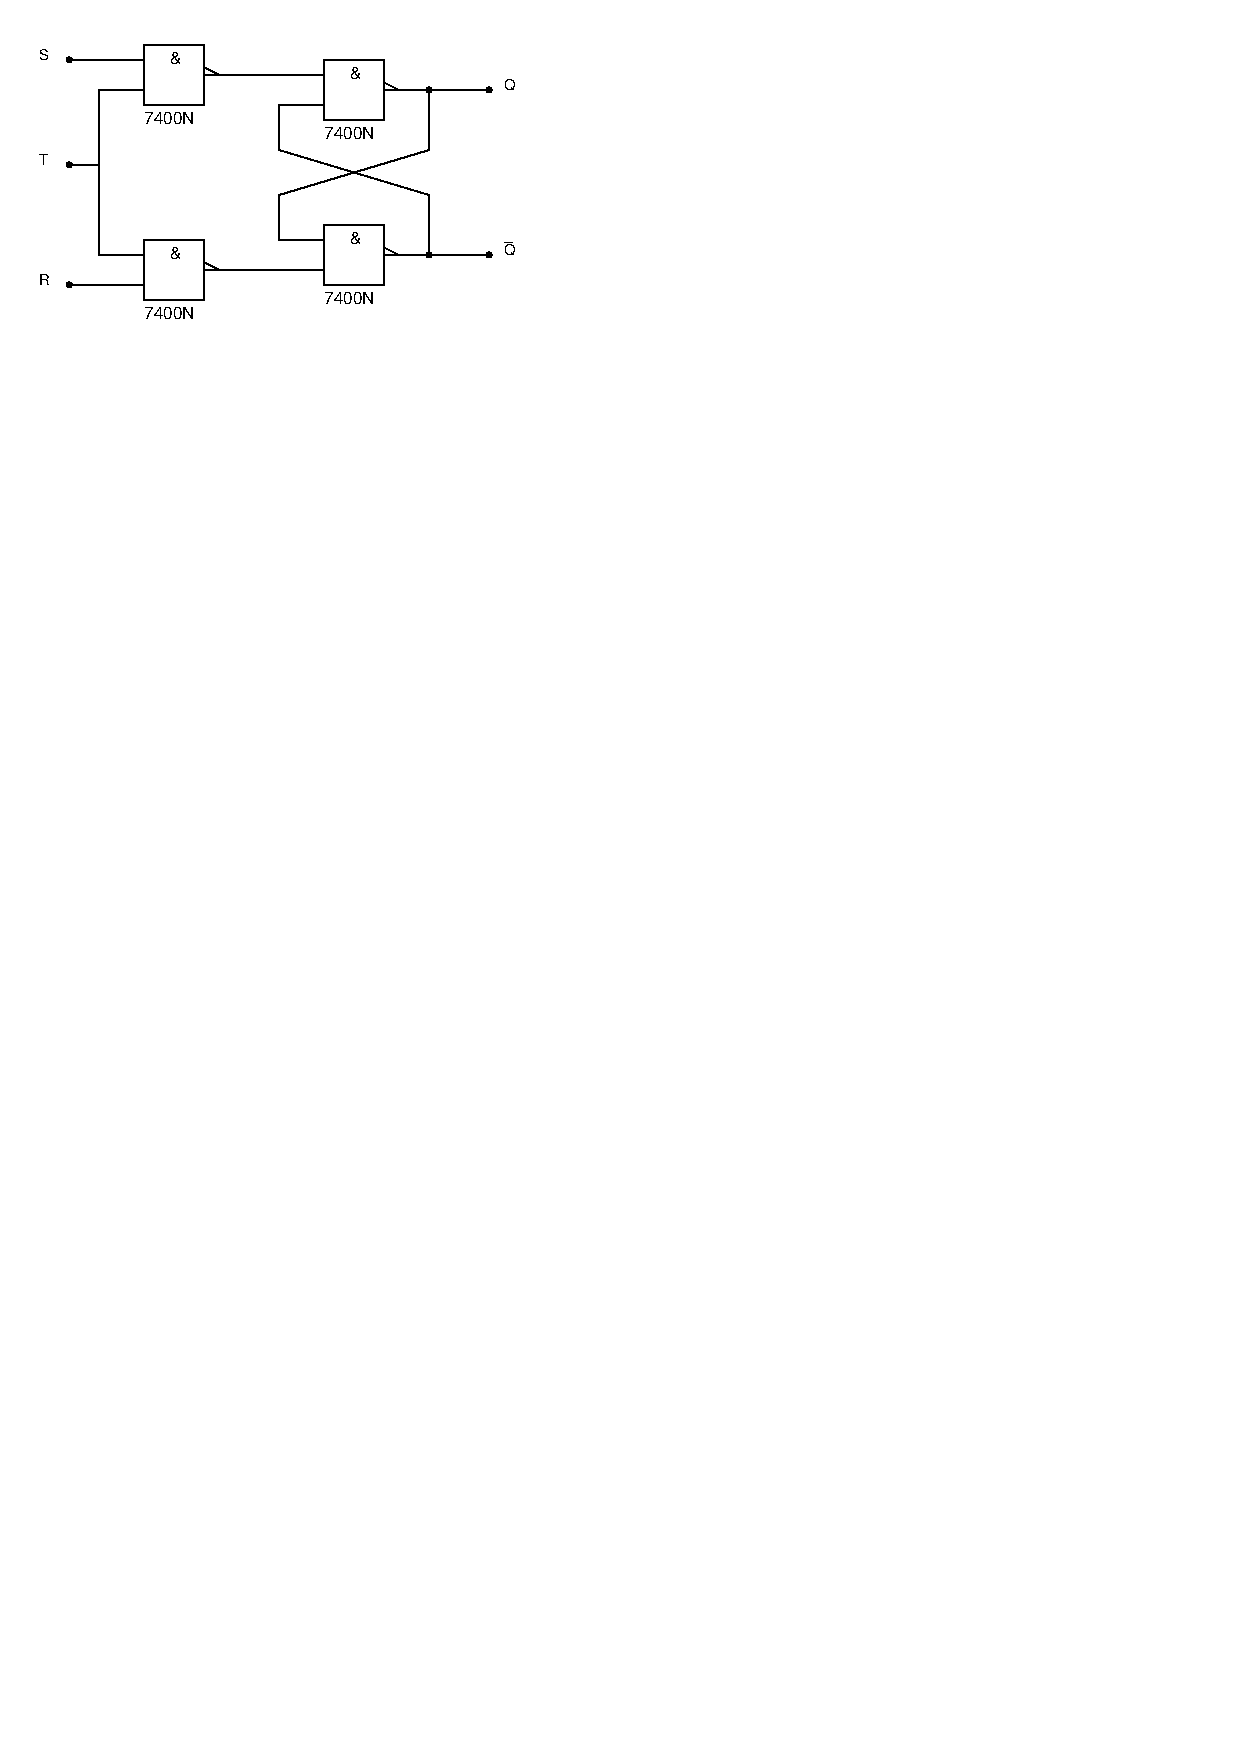
\includegraphics[height=6cm]{Schaltplaene/42_Getaktetes_RS-Flip-Flop.pdf}\end{center}
\begin{center}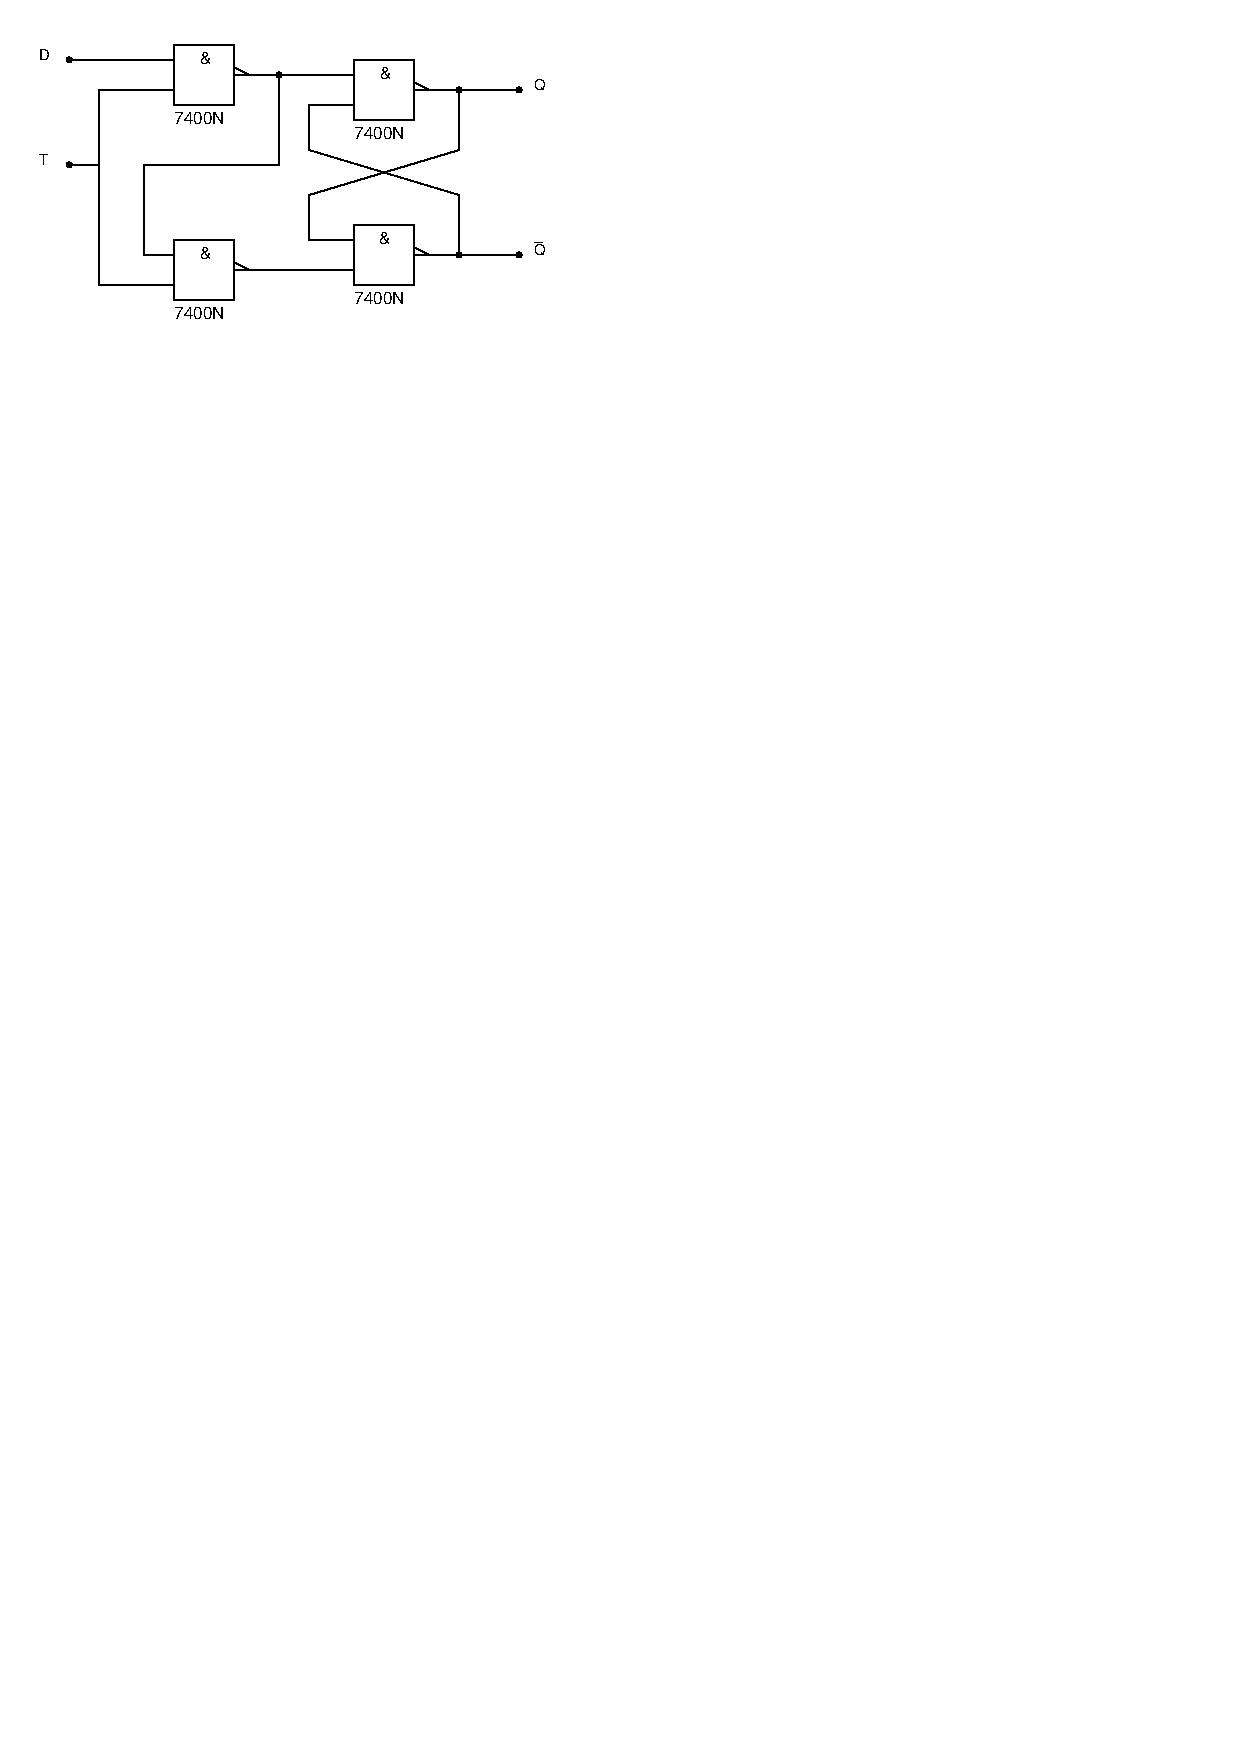
\includegraphics[height=6cm]{Schaltplaene/41b_D-Flip-Flop.pdf}\end{center}
\subsection*{4.3 JK-MS-Flip-Flop}
\begin{center}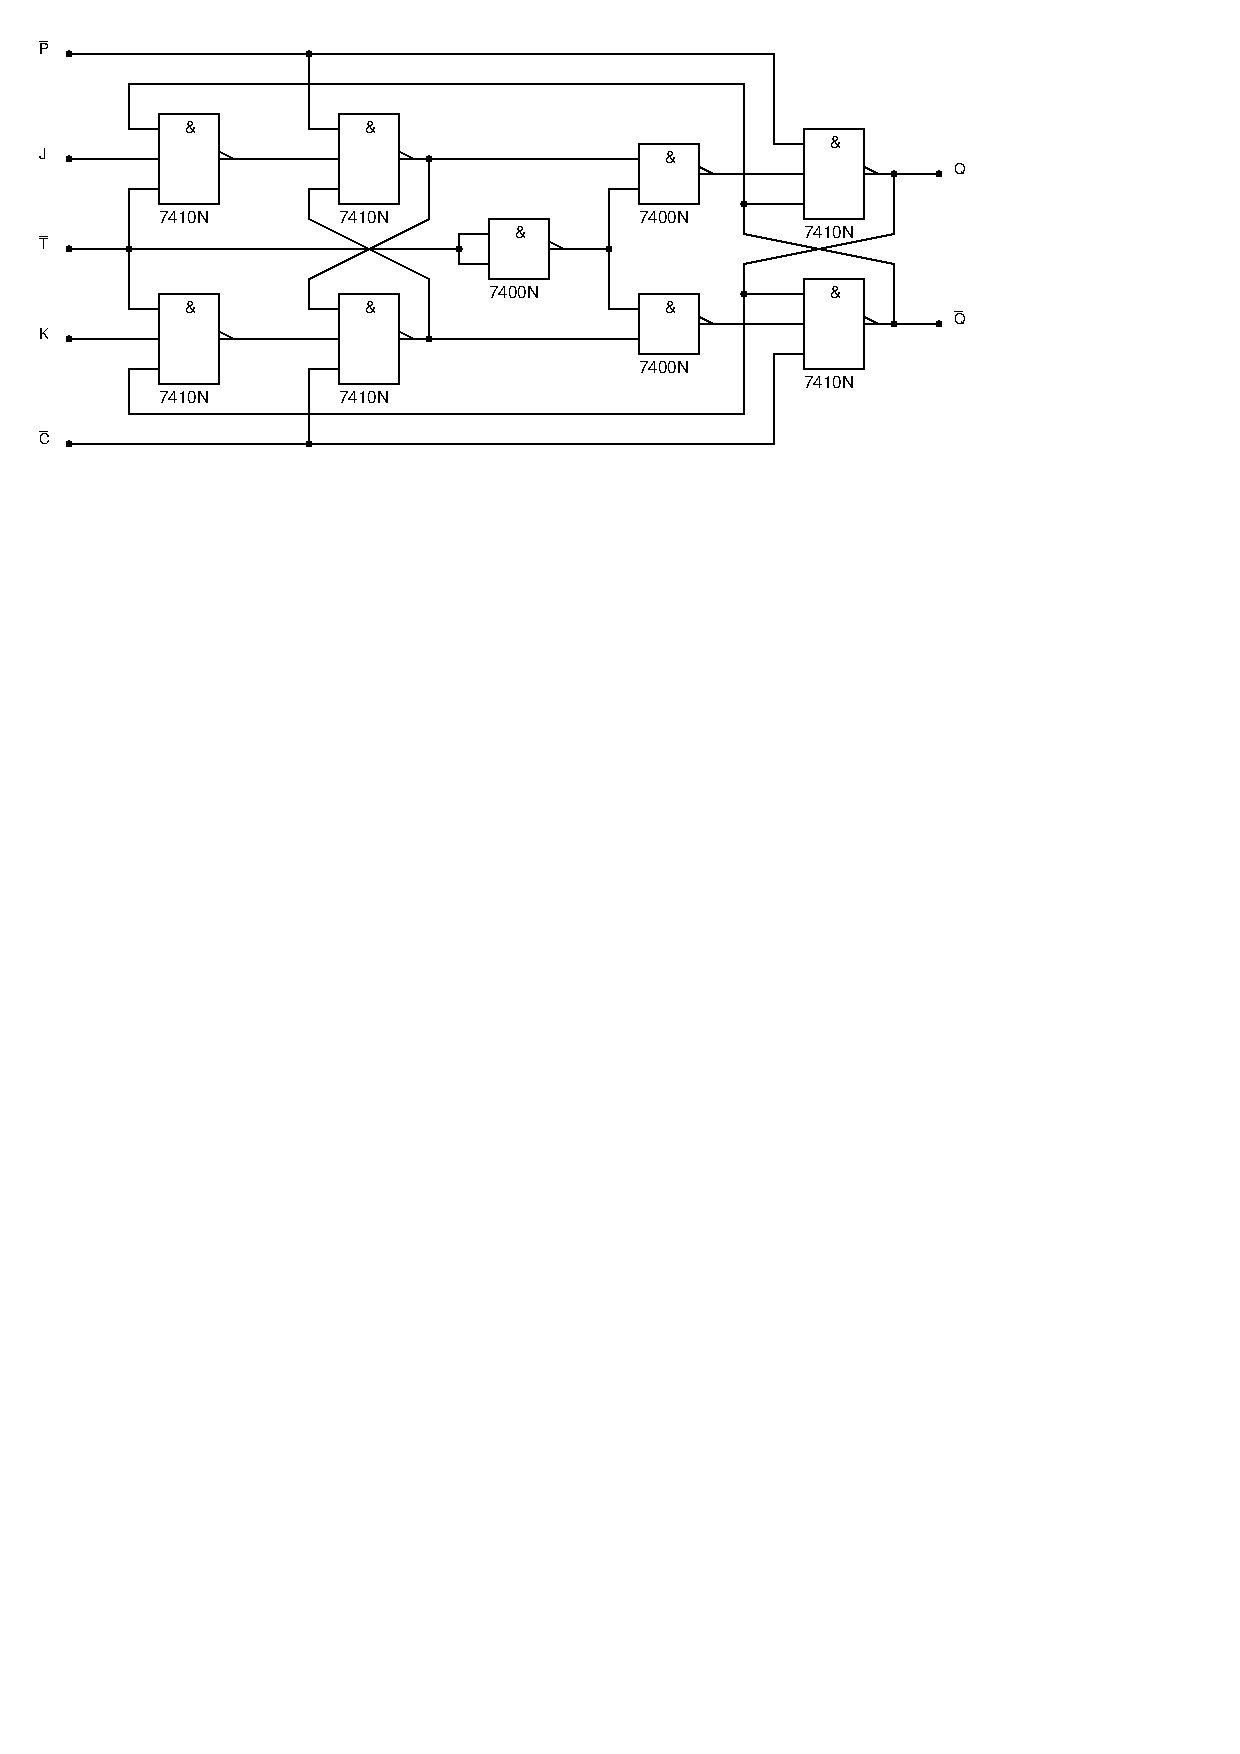
\includegraphics[width=15cm]{Schaltplaene/43_JK_Master-Slave-Flip-Flop.pdf}\end{center}
\subsection*{5.1 Schieberegister}
\begin{center}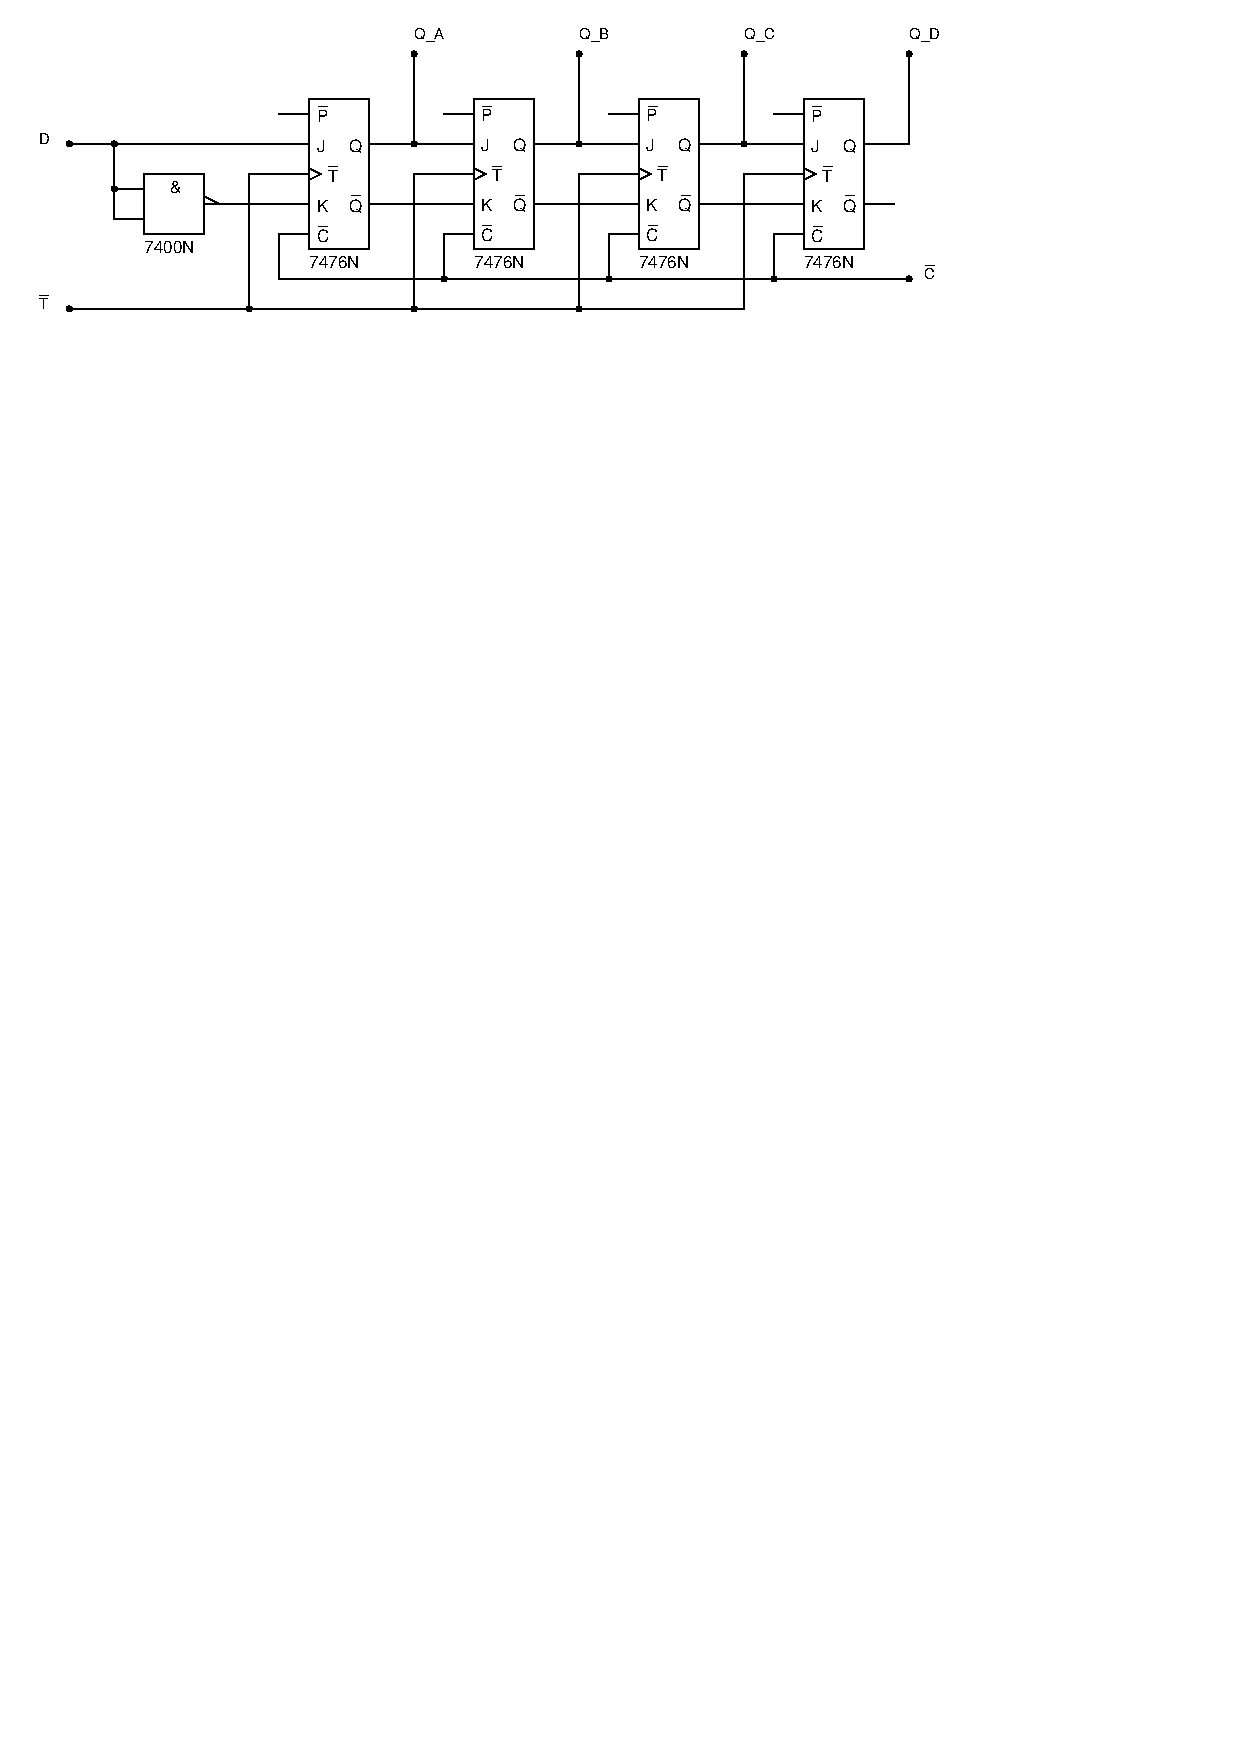
\includegraphics[width=15cm]{Schaltplaene/51_Schieberegister.pdf}\end{center}
\subsection*{5.2 Rotationsregister}
\begin{center}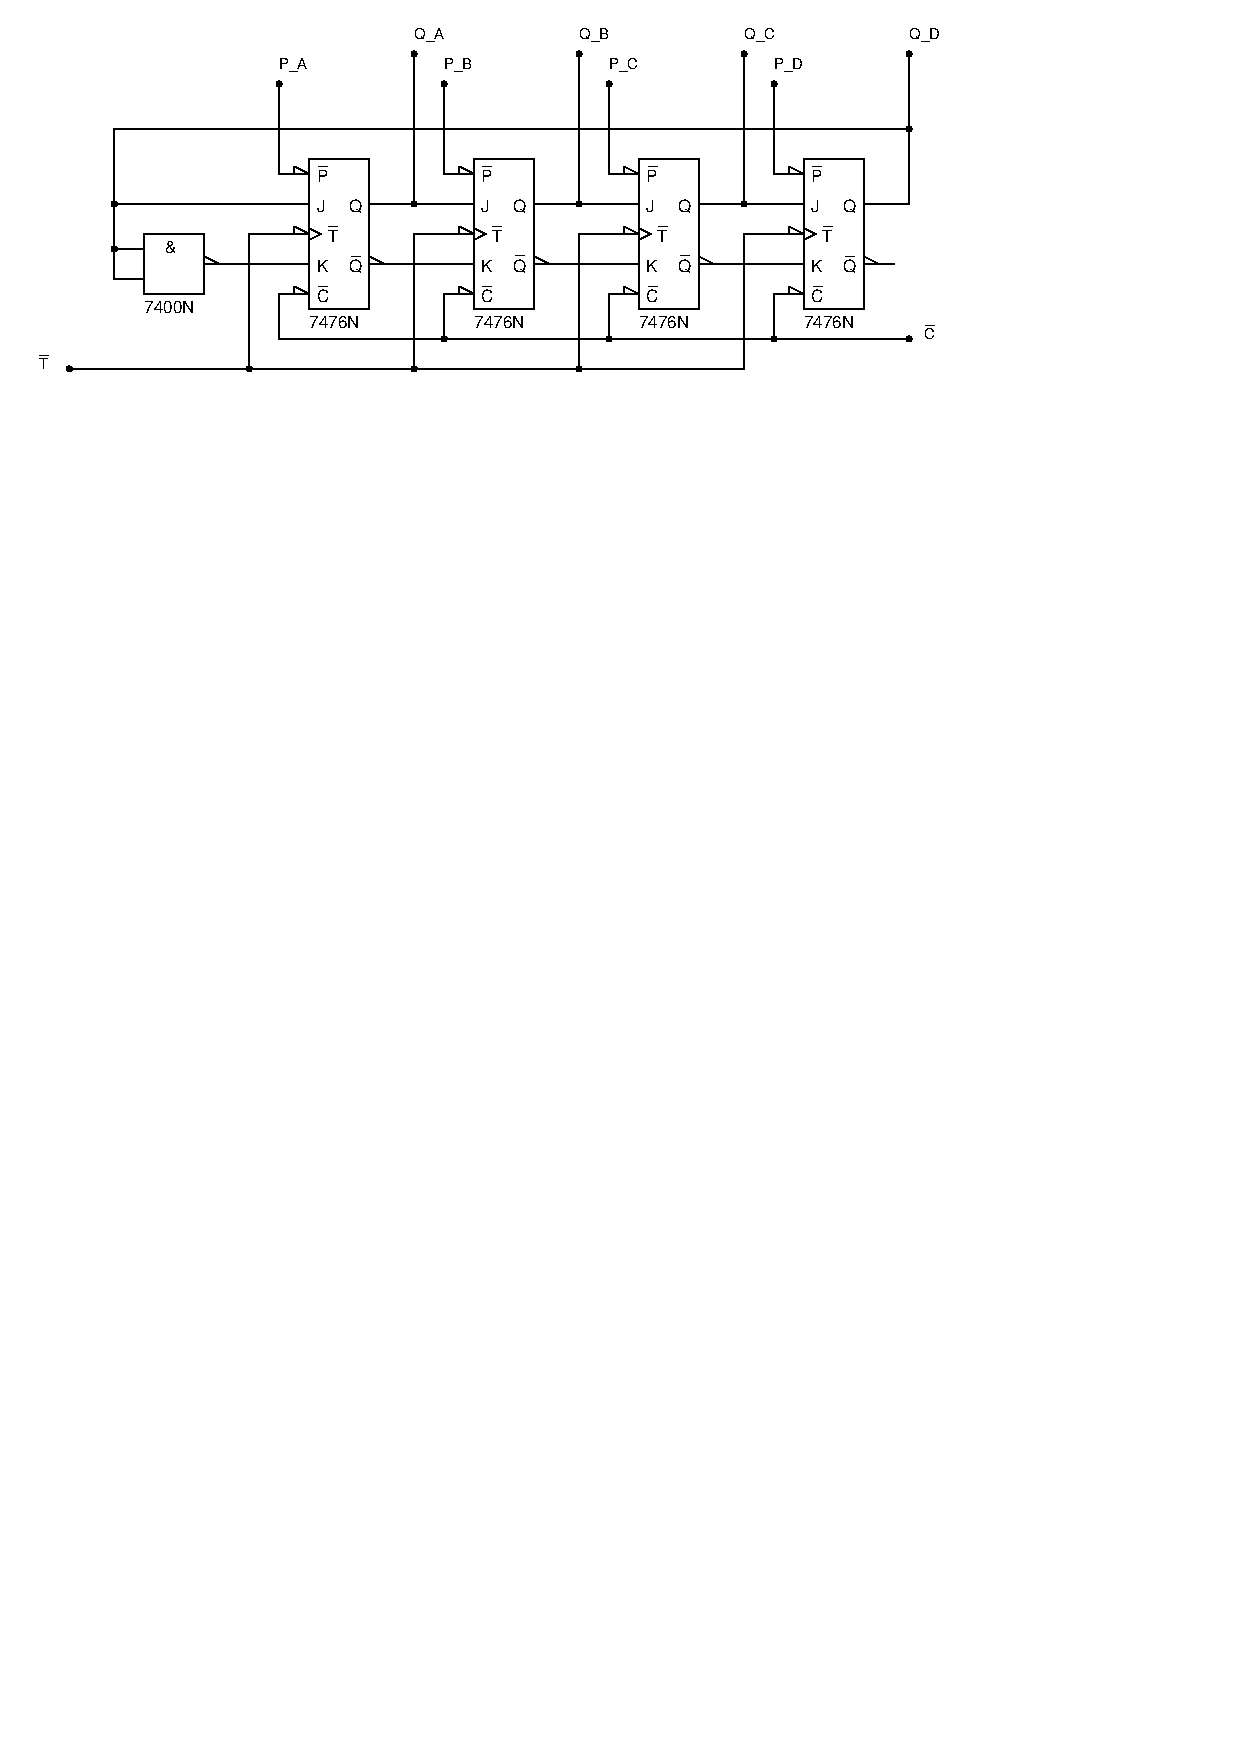
\includegraphics[width=15cm]{Schaltplaene/52_Rotationsregister.pdf}\end{center}
\subsection*{6.1 Asynchronz�hler}
\begin{center}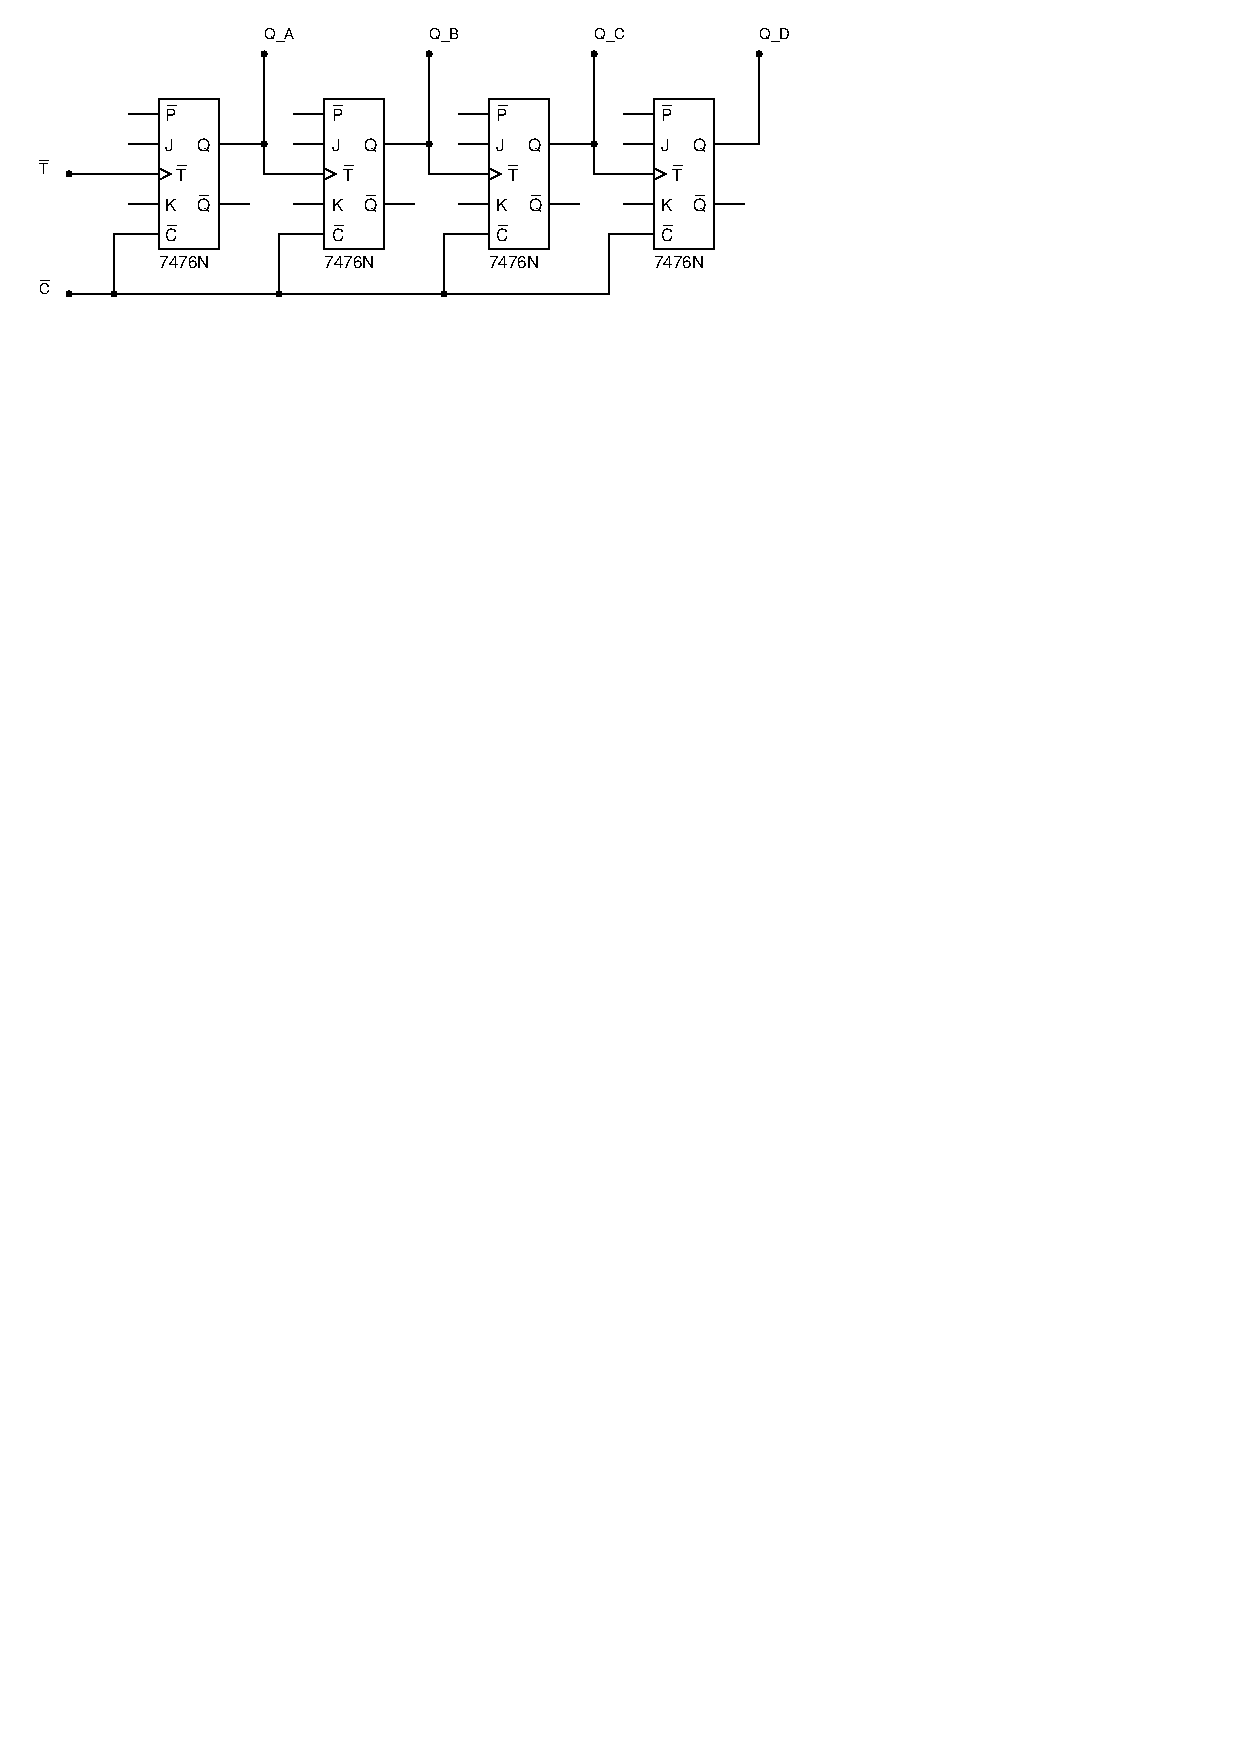
\includegraphics[width=15cm]{Schaltplaene/61_4-Bit_Asynchronzaehler.pdf}\end{center}
\begin{center}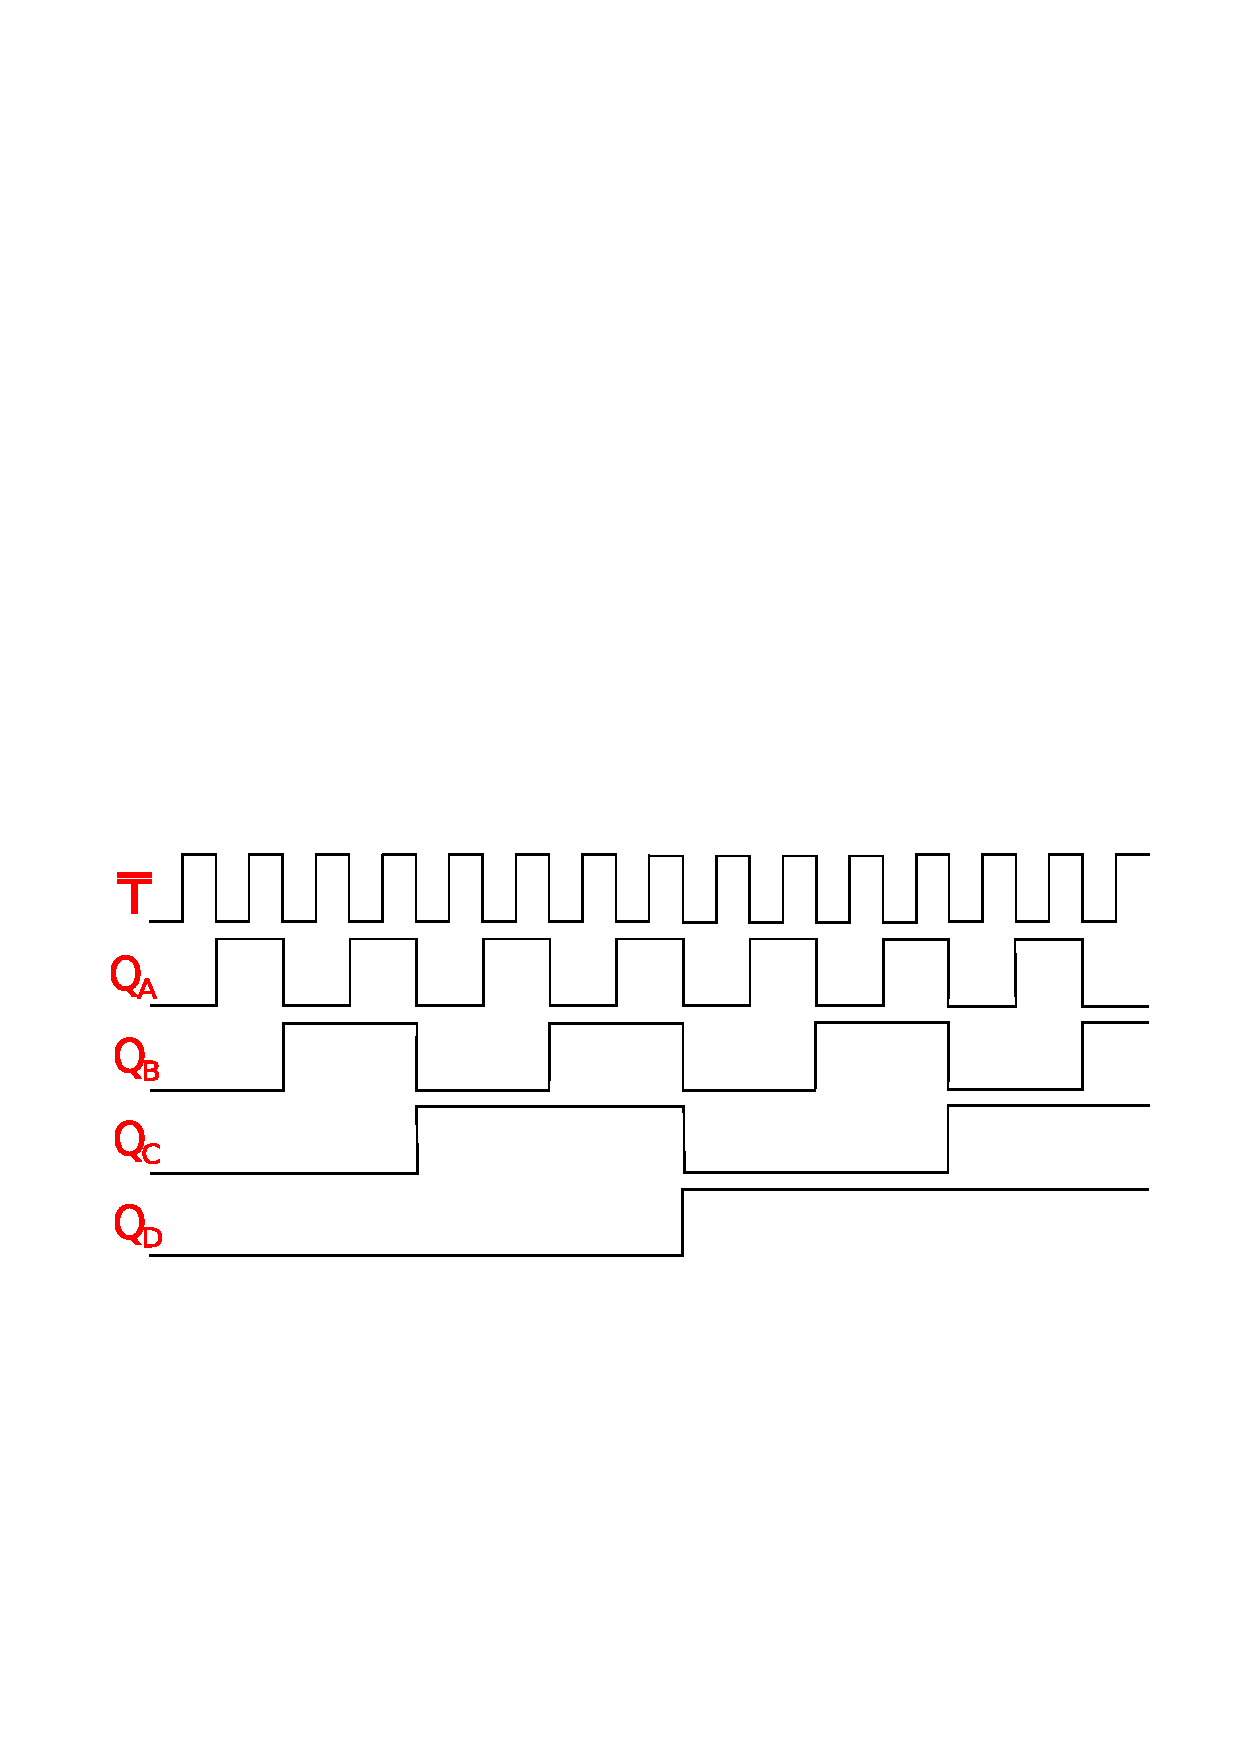
\includegraphics[width=10cm]{Bilder/zaehler.pdf}\end{center}
\subsection*{6.2 Asynchroner Dezimalz�hler}
\begin{center}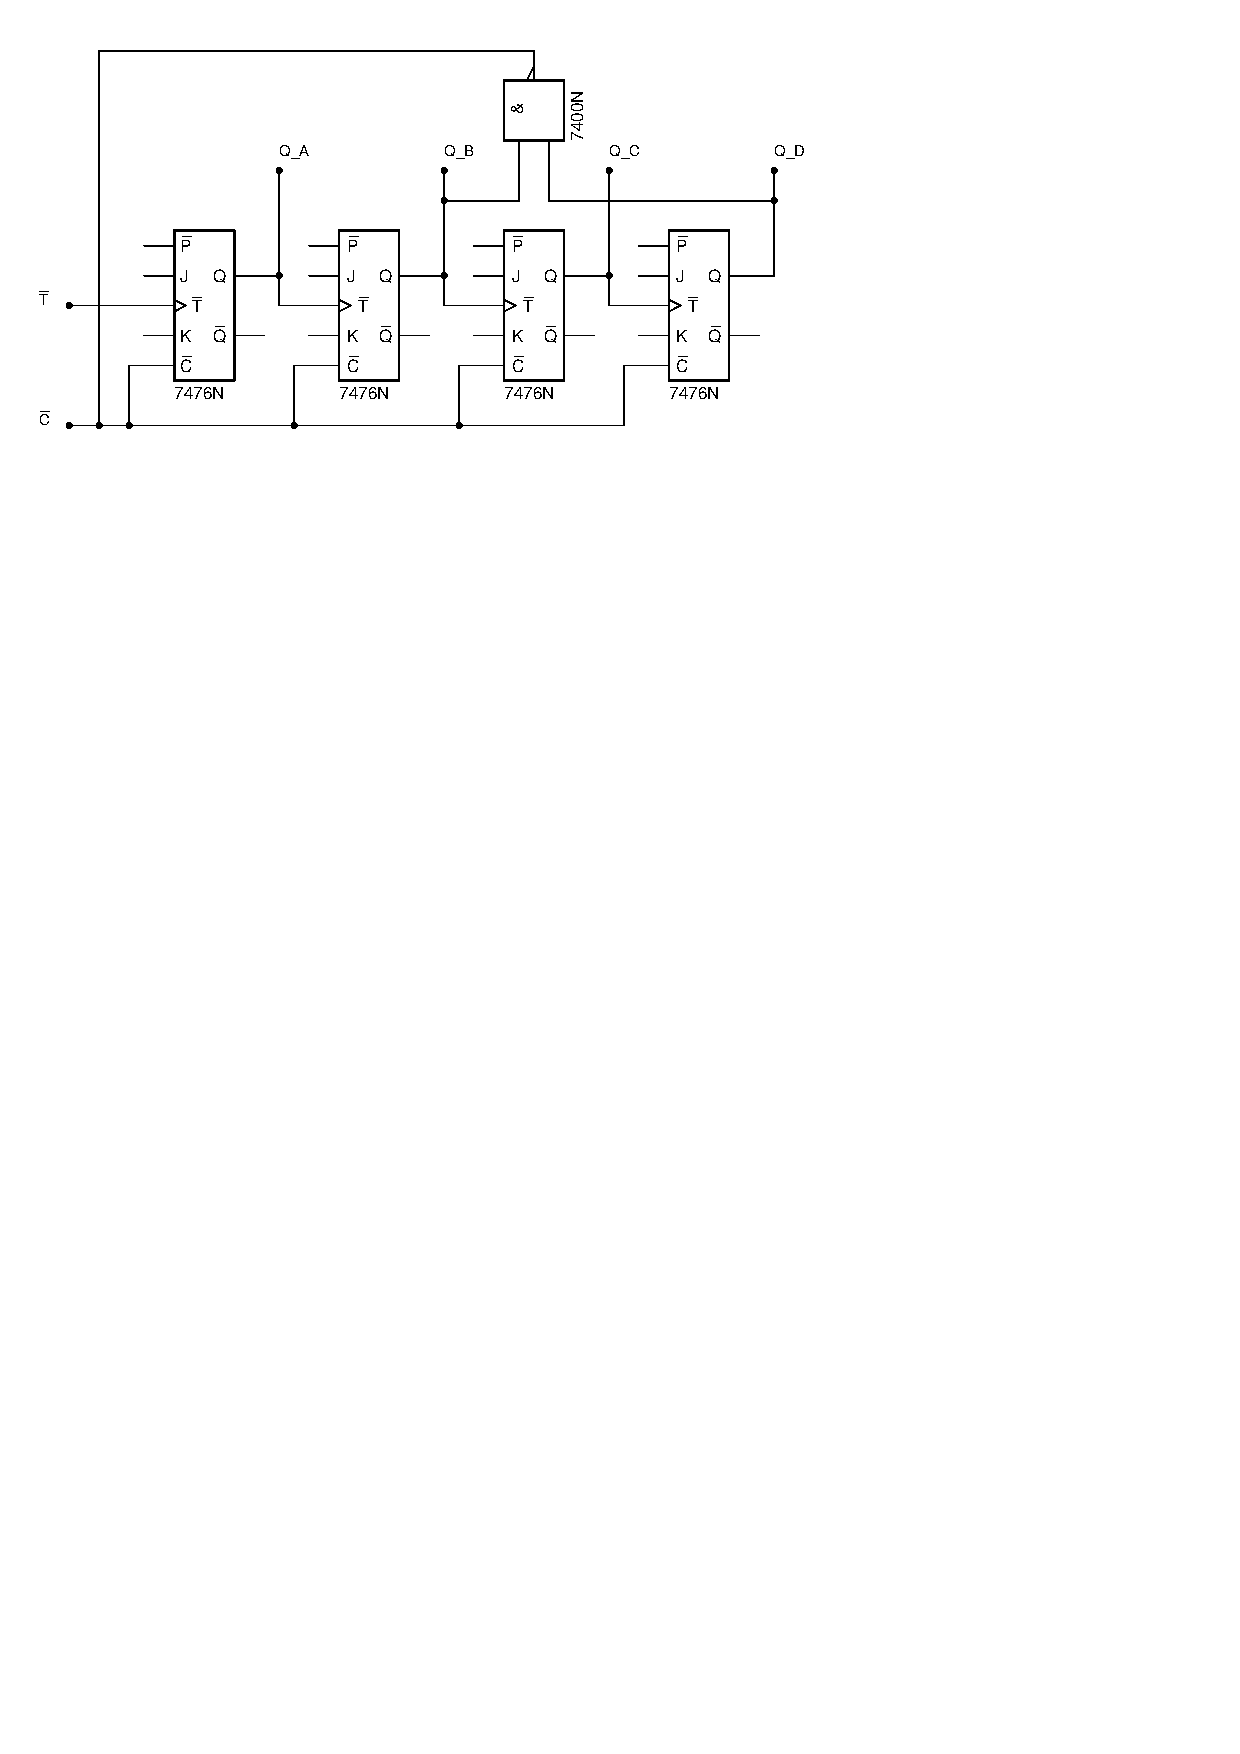
\includegraphics[width=15cm]{Schaltplaene/62_Dezimaler_Asynchronzaehler.pdf}\end{center}
\subsection*{6.3 Synchronz�hler}
\begin{center}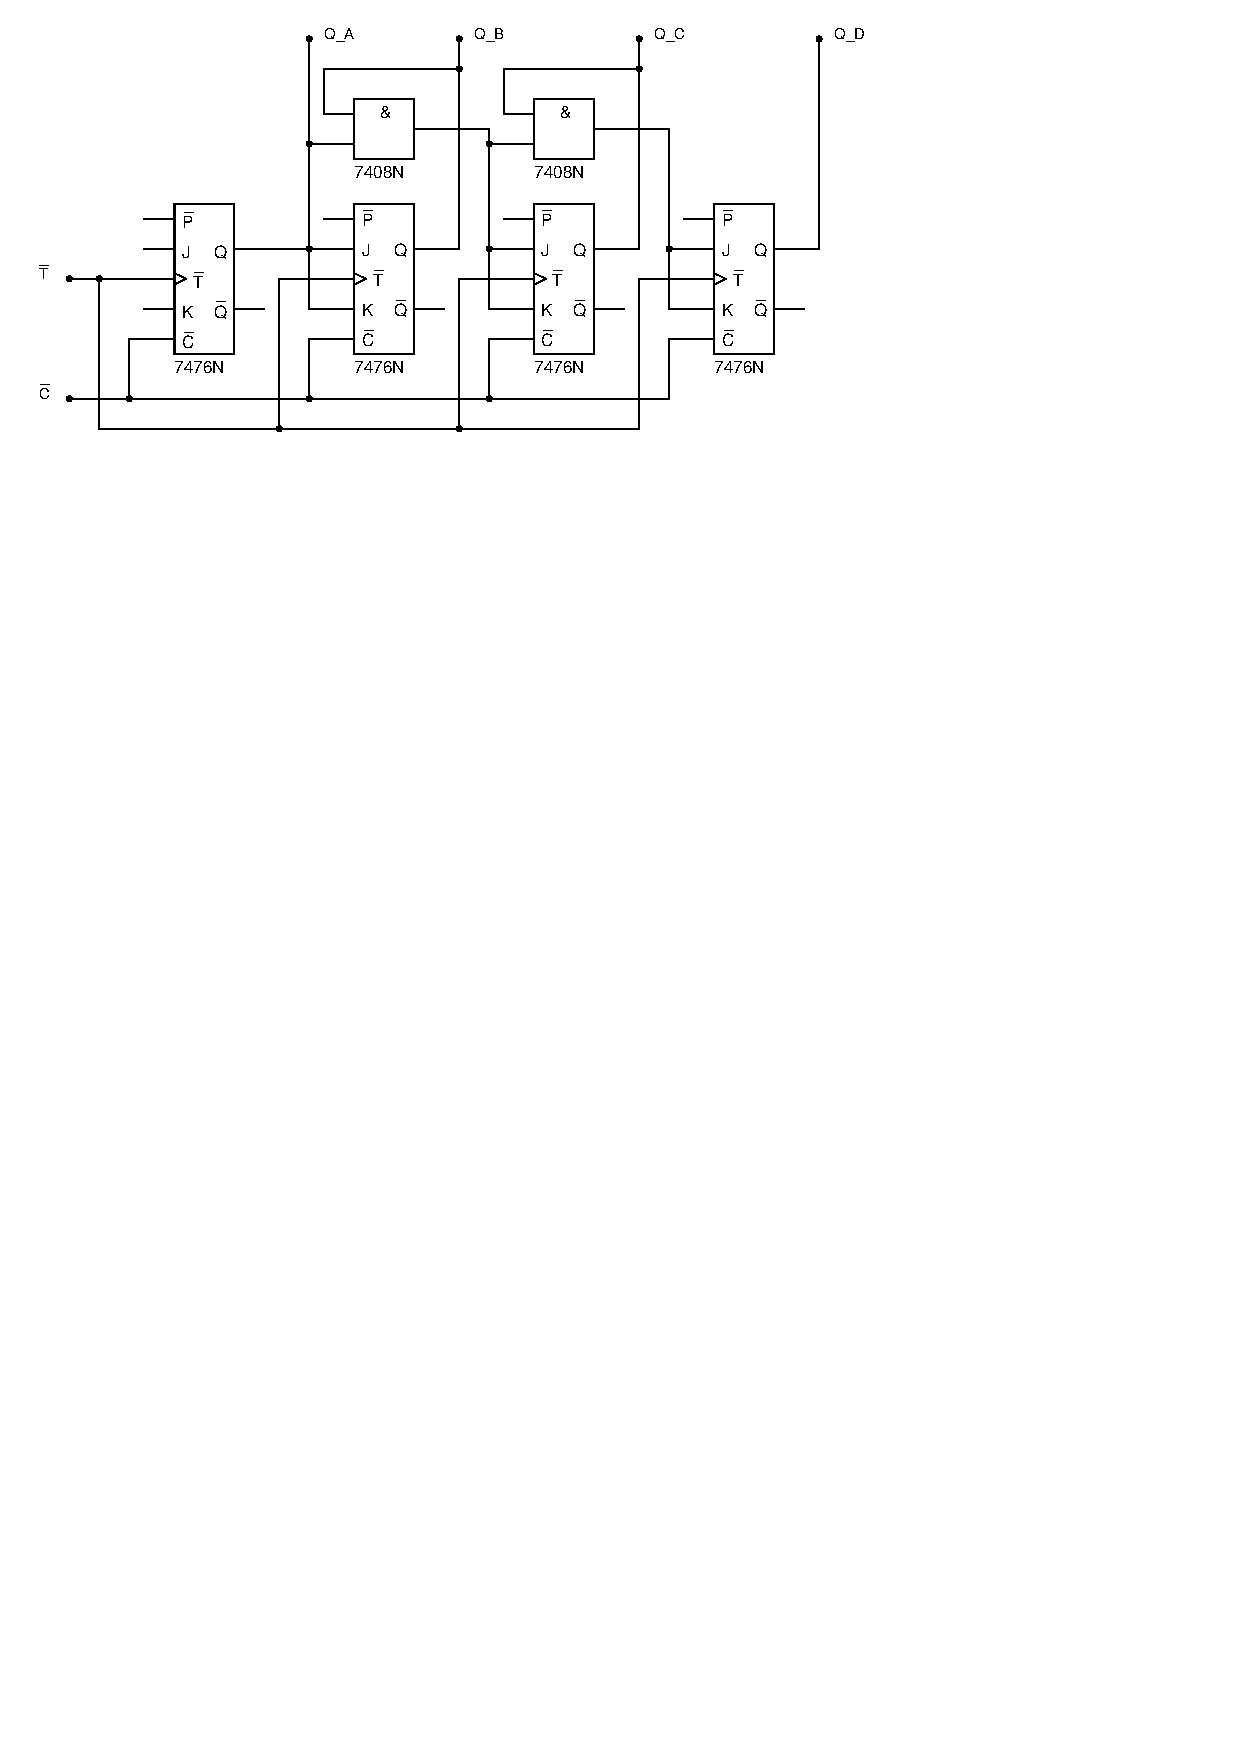
\includegraphics[width=15cm]{Schaltplaene/63_Dualer_Synchronzaehler.pdf}\end{center}
\subsection*{6.4 Synchroner Dezimalz�hler}
\begin{center}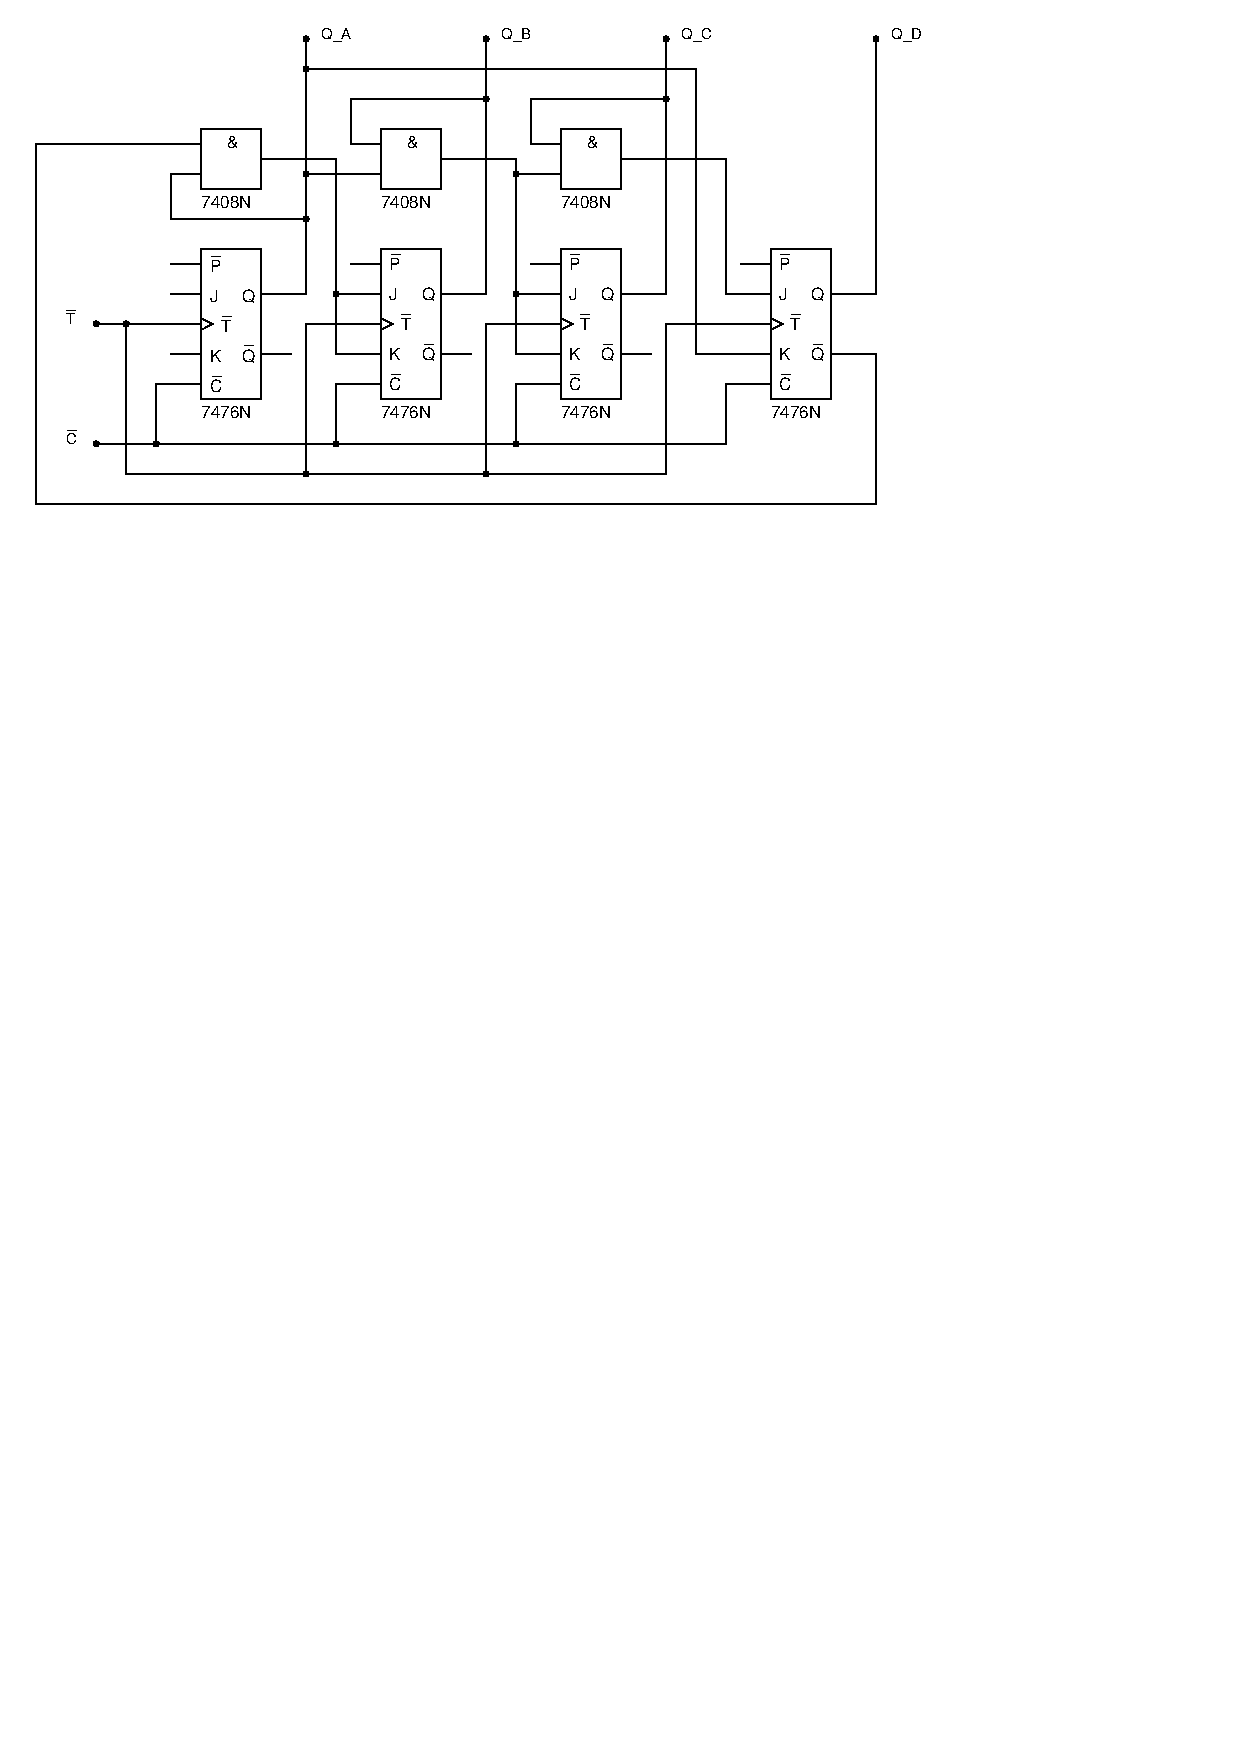
\includegraphics[width=15cm]{Schaltplaene/64_Dezimaler_Synchronzaehler.pdf}\end{center}
\subsection*{7 Digital-nach-Analog-Wandlung}
\begin{center}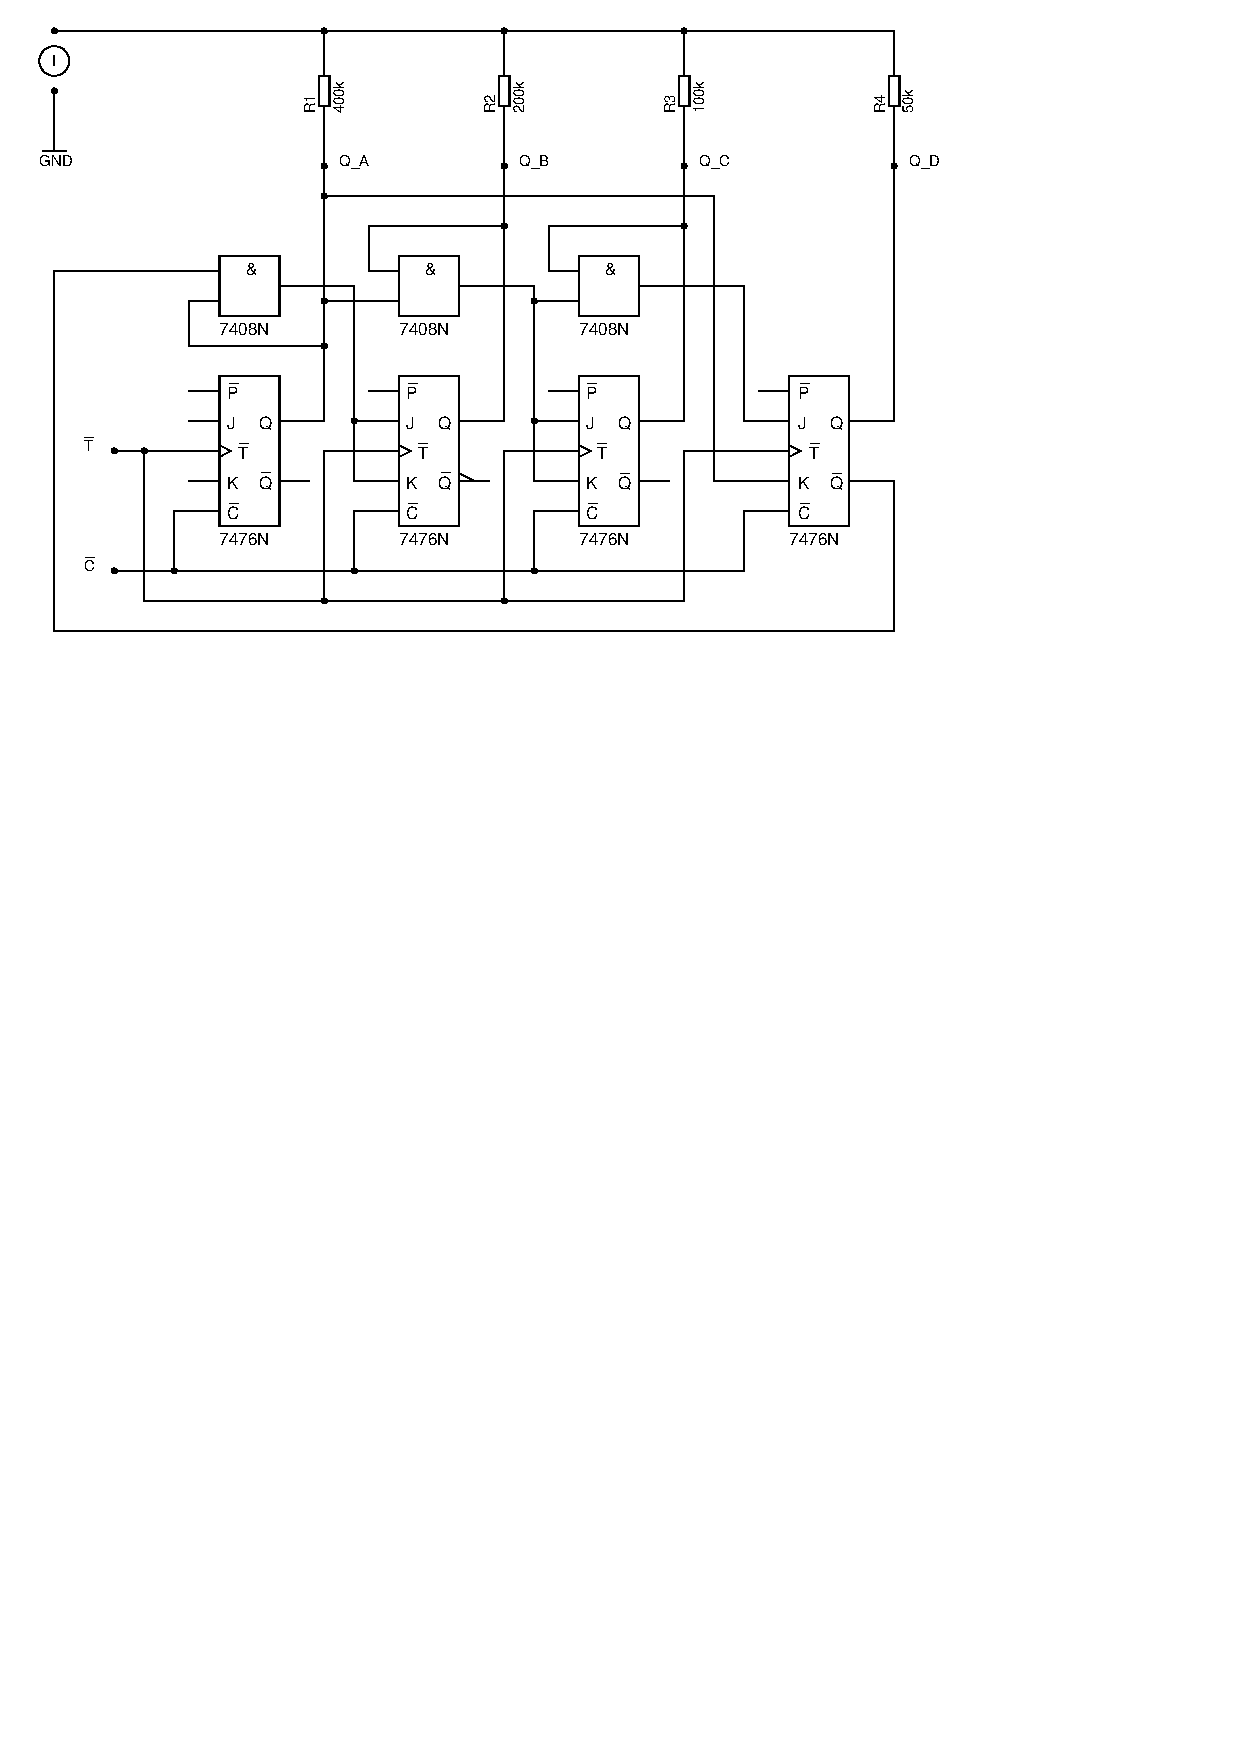
\includegraphics[width=15cm]{Schaltplaene/70_Dezimaler_Synchronzaehler_-_Digital-Analogwandlung.pdf}\end{center}
\end{document}
